\documentclass[11pt]{article}

\usepackage[margin=1in]{geometry}
\usepackage{graphicx}
\usepackage{booktabs}
\usepackage{longtable}
\usepackage{array}
\usepackage[strings]{underscore}
\usepackage{hyperref}
\usepackage{xcolor}
\usepackage{amssymb}
\usepackage{enumitem}
\usepackage{float}
\usepackage{fvextra}
\usepackage{tikz}
\usetikzlibrary{arrows.meta,positioning}

\hypersetup{
  colorlinks=true,
  linkcolor=blue,
  urlcolor=blue,
  citecolor=blue
}

\setlist[itemize]{leftmargin=1.5em}

\newcommand{\code}[1]{\texttt{#1}}
\newcommand{\checked}{\texttt{[x]}}
\newcommand{\unchecked}{\texttt{[ ]}}
\newcommand{\statusverified}{\textbf{Verified}}
\newcommand{\statusunverified}{\textbf{Unverified}}

\title{Final E2E Report (Evidence-Based)\\Real-Time Fraud Detection ML System}
\author{Repository: \code{Final_Project_DMM501_Group1}}
\date{2026-04-14}

\begin{document}
\maketitle
\tableofcontents
\newpage

\section{Evidence Pack (What was extracted)}
All metrics and file references are from this repository and the generated outputs under \code{artifacts/}. If a component was not executed live during report generation, it is marked \statusunverified{}.

\subsection{Dataset evidence (Kaggle credit card fraud)}
\begin{itemize}
  \item Dataset file in repo: \code{data/archive/creditcard.csv}
  \item Schema validation: \code{artifacts/reports/dataset_schema.json}
  \item EDA summary: \code{artifacts/reports/eda_summary.json}
  \item Class imbalance: \code{artifacts/reports/class_distribution.json}
  \item EDA figures: \code{artifacts/figures/*.png}
\end{itemize}

\subsection{Model artifacts (deployable model + metadata)}
\begin{itemize}
  \item Deployable model: \code{artifacts/models/final_model.joblib}
  \item Deploy metadata: \code{artifacts/models/model_info.json}
  \item Model selection summary: \code{artifacts/reports/model_selection_summary.json}
  \item Model validation checks: \code{artifacts/reports/model_validation_checks.json}
\end{itemize}

\subsection{Evaluation and explainability figures}
\begin{itemize}
  \item ROC/PR curves: \code{artifacts/figures/baseline_*}, \code{artifacts/figures/improved_*}
  \item Threshold tuning: \code{artifacts/figures/*threshold*}, \code{artifacts/benchmarks/*threshold*}
  \item Model comparison: \code{artifacts/figures/model_comparison.png}
  \item SHAP: \code{artifacts/figures/shap_summary.png}, \code{artifacts/benchmarks/shap_importance_table.csv}
\end{itemize}

\subsection{Frontend evidence}
\begin{itemize}
  \item UI layout: \code{frontend/index.html}
  \item Streaming logic + risk classification: \code{frontend/app.js}
  \item API client (timeouts + schema assertions): \code{frontend/api-client.js}
  \item Transaction sources: \code{frontend/demo-data.js}, \code{frontend/real-samples.json}
  \item UI screenshot (layout evidence): \code{artifacts/figures/frontend_dashboard_live.png}
\end{itemize}

\subsection{API evidence}
\begin{itemize}
  \item FastAPI app: \code{src/api/main.py}
  \item Schemas: \code{src/api/schemas.py}
  \item Model loader: \code{src/models/loader.py}
  \item Dataset sampling: \code{src/data/samples.py}
  \item Metrics: \code{src/monitoring/metrics.py}
  \item Verification harness: \code{verify_system.py} (\statusunverified{} run in this report)
\end{itemize}

\subsection{Monitoring and deployment evidence}
\begin{itemize}
  \item Compose stack: \code{deployment/docker-compose.yml}
  \item Prometheus: \code{deployment/prometheus/prometheus.yml}, \code{deployment/prometheus/alerts.yml}
  \item Grafana: \code{deployment/grafana/dashboards/fraud_api.json} + provisioning
  \item CI/CD: \code{.github/workflows/ci.yml}, \code{.github/workflows/docker.yml}
\end{itemize}

\section{Problem Definition}
\subsection{Problem statement}
Build an end-to-end ML system that assigns a fraud risk score to credit-card transactions and serves predictions via an API, with a demo dashboard for near-real-time monitoring and an observability stack (metrics, dashboards, alerting).

\subsection{Business context}
Fraud scoring reduces financial loss and manual review cost by prioritizing transactions for investigation. In this system, the decision threshold is treated as an explicit operational policy (stored as model metadata and returned in API responses).

\section{Dataset Analysis (with imbalance explanation)}
\subsection{Schema (evidence)}
From \code{artifacts/reports/dataset_schema.json}: the dataset has 284,807 rows and 31 columns: \code{Time}, \code{V1..V28}, \code{Amount}, \code{Class} (\code{matches_expected_schema=true}).

\subsection{Imbalance (evidence)}
From \code{artifacts/reports/class_distribution.json}:
\begin{itemize}
  \item Class 0 (non-fraud): 284,315 (ratio=0.9982725144; \(\approx 99.8273\%\))
  \item Class 1 (fraud): 492 (ratio=0.0017274856; \(\approx 0.1727\%\))
\end{itemize}
\textbf{Why accuracy is misleading:} With a 0.17\% fraud rate, a naive model predicting ``non-fraud'' for every transaction achieves \(\approx 99.83\%\) accuracy. Therefore, this project emphasizes PR-AUC and precision/recall at an operating threshold.

\subsection{Data quality notes (evidence)}
From \code{artifacts/reports/eda_summary.json}: duplicate rows = 1081. Missing value counts are exported to \code{artifacts/reports/missing_values.csv}.
Figures \ref{fig:class_dist}, \ref{fig:amount_dist}, and \ref{fig:time_dist} summarize the imbalance and transaction distributions used as input assumptions for model and threshold selection.

\subsection{Embedded dataset figures}
\begin{figure}[H]
  \centering
  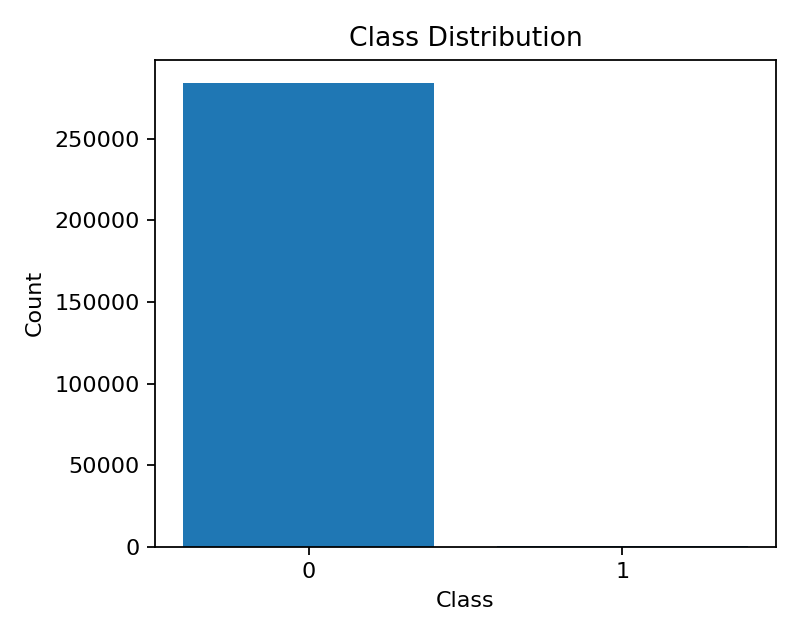
\includegraphics[width=0.75\linewidth]{../artifacts/figures/class_distribution.png}
  \caption{Class distribution (Fraud vs Non-fraud). Source: \code{artifacts/figures/class_distribution.png}}
  \label{fig:class_dist}
\end{figure}
\begin{figure}[H]
  \centering
  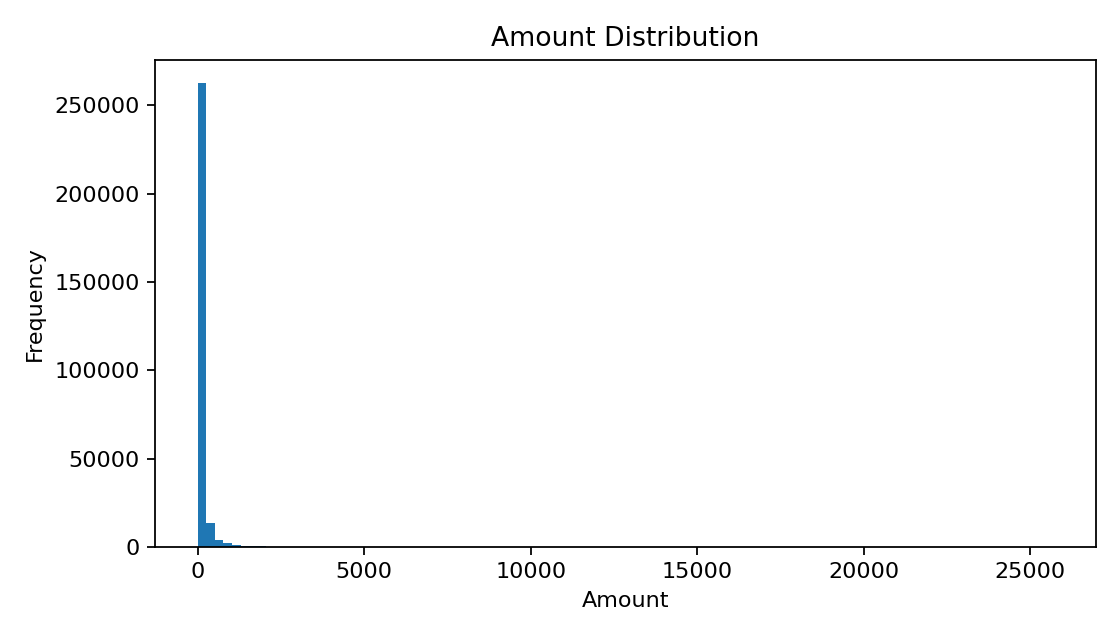
\includegraphics[width=0.85\linewidth]{../artifacts/figures/amount_distribution.png}
  \caption{Amount distribution. Source: \code{artifacts/figures/amount_distribution.png}}
  \label{fig:amount_dist}
\end{figure}
\begin{figure}[H]
  \centering
  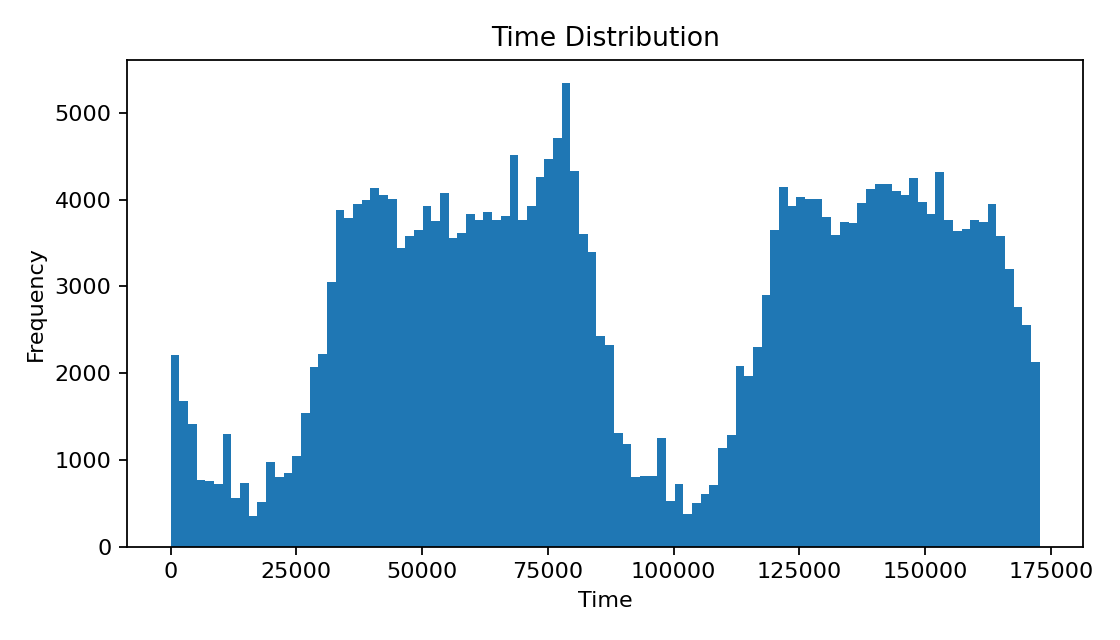
\includegraphics[width=0.85\linewidth]{../artifacts/figures/time_distribution.png}
  \caption{Time distribution. Source: \code{artifacts/figures/time_distribution.png}}
  \label{fig:time_dist}
\end{figure}
\begin{figure}[H]
  \centering
  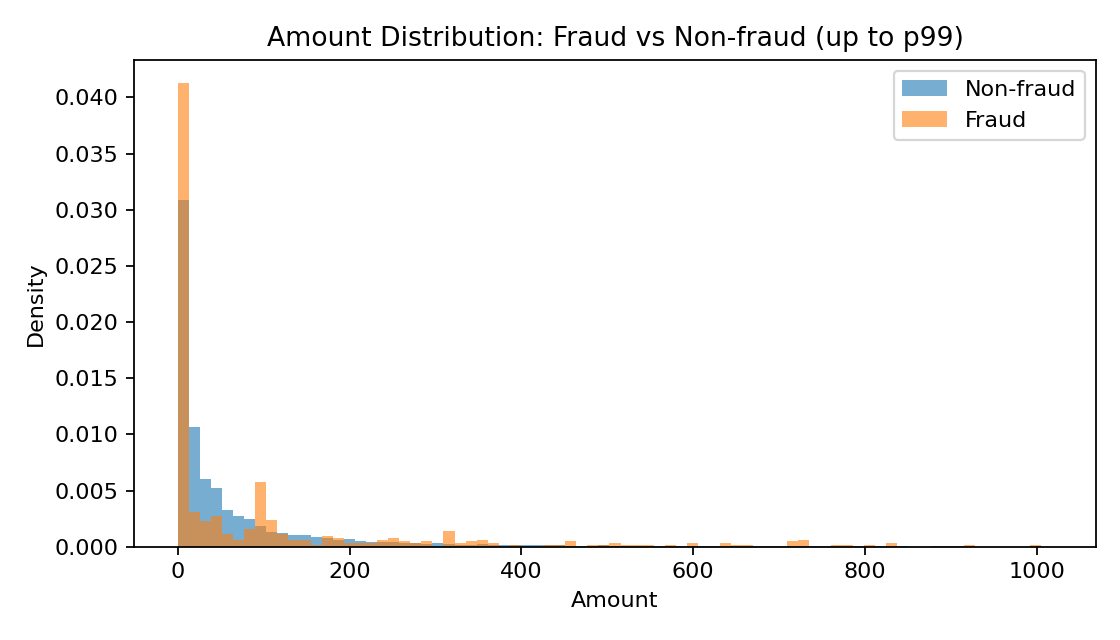
\includegraphics[width=0.85\linewidth]{../artifacts/figures/fraud_vs_nonfraud_amount.png}
  \caption{Fraud vs non-fraud amount patterns. Source: \code{artifacts/figures/fraud_vs_nonfraud_amount.png}}
  \label{fig:fraud_amount}
\end{figure}
\begin{figure}[H]
  \centering
  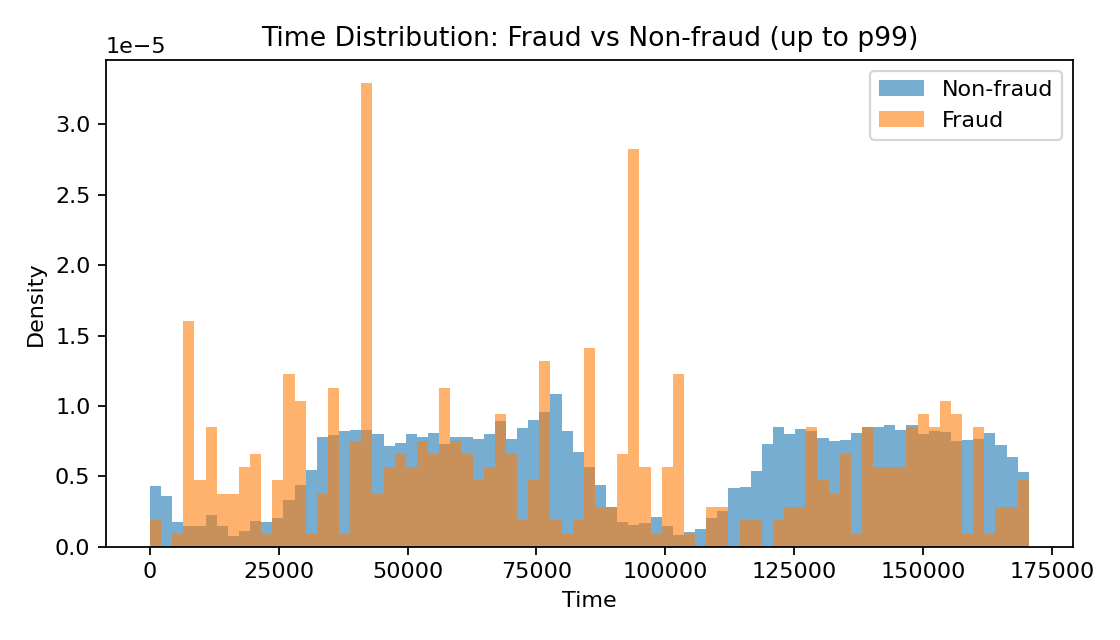
\includegraphics[width=0.85\linewidth]{../artifacts/figures/fraud_vs_nonfraud_time.png}
  \caption{Fraud vs non-fraud time patterns. Source: \code{artifacts/figures/fraud_vs_nonfraud_time.png}}
  \label{fig:fraud_time}
\end{figure}
\begin{figure}[H]
  \centering
  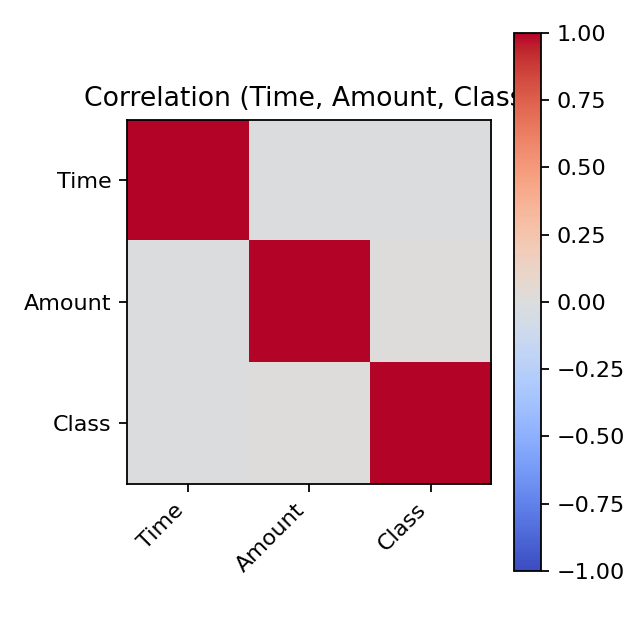
\includegraphics[width=0.9\linewidth]{../artifacts/figures/correlation_overview.png}
  \caption{Feature correlation overview. Source: \code{artifacts/figures/correlation_overview.png}}
  \label{fig:corr_overview}
\end{figure}

\section{ML Pipeline}
\subsection{Primary pipeline}
The primary benchmark pipeline is implemented in \code{src/pipelines/run_model_workflow.py}. It performs:
\begin{itemize}
  \item dataset schema validation and EDA exports
  \item train/val/test split (seeded)
  \item baseline training (Logistic Regression pipeline)
  \item improved training (LightGBM with small hyperparameter sweep)
  \item threshold tuning (validation sweep; best by max F1)
  \item evaluation exports (ROC/PR, confusion matrices, classification reports)
  \item SHAP explainability exports for LightGBM
  \item model selection (primary criterion PR-AUC) and deployable artifact export
\end{itemize}

\subsection{Split (evidence)}
From \code{artifacts/reports/split_info.json}:
train=199,364; val=42,721; test=42,722; n\_features=30; seed=42.

\section{Model Training (baseline vs improved)}
\subsection{Models implemented}
\begin{itemize}
  \item Baseline: scikit-learn \code{Pipeline(StandardScaler, LogisticRegression)} with \code{class_weight="balanced"}.
  \item Improved: \code{lightgbm.LGBMClassifier} tuned by validation PR-AUC across a small \code{ParameterGrid}. Hyperparameter results: \code{artifacts/benchmarks/improved_hyperparameter_tuning.csv}.
\end{itemize}

\subsection{Best LightGBM hyperparameters (evidence)}
From the top row of \code{artifacts/benchmarks/improved_hyperparameter_tuning.csv} (sorted by \code{val_pr_auc}):
\begin{itemize}
  \item \code{val_pr_auc}=0.62893
  \item \code{learning_rate}=0.03, \code{n_estimators}=450, \code{num_leaves}=63
  \item \code{scale_pos_weight}=10.0 (natural ratio recorded as \(\approx 578.55\))
\end{itemize}

\subsection{Metrics table (evidence)}
From \code{artifacts/reports/model_selection_summary.json}:

\begin{table}[H]
  \centering
  \begin{tabular}{lrrrrrrrrrr}
    \toprule
    Model & Thr & PR-AUC & ROC-AUC & Prec & Rec & F1 & TN & FP & FN & TP \\
    \midrule
    Logistic Regression (baseline) & 0.99 & 0.7929 & 0.9680 & 0.6742 & 0.8108 & 0.7362 & 42619 & 29 & 14 & 60 \\
    LightGBM (improved) & 0.84 & 0.7161 & 0.8828 & 0.8852 & 0.7297 & 0.8000 & 42641 & 7 & 20 & 54 \\
    \bottomrule
  \end{tabular}
  \caption{Tuned test metrics (evidence). Source: \code{artifacts/reports/model_selection_summary.json}}
\end{table}

\subsection{Additional test-set evidence (accuracy and supports)}
From \code{artifacts/reports/baseline_classification_report.json} and \code{artifacts/reports/improved_classification_report.json}:
\begin{itemize}
  \item Test set supports: non-fraud=42648, fraud=74
  \item Baseline accuracy: 0.99899349
  \item Improved accuracy: 0.99936801
\end{itemize}
\textbf{Interpretation:} Accuracy is high for both models due to extreme imbalance; this repo uses PR-AUC and tuned precision/recall as primary evidence.

\subsection{Model selection (deployable choice)}
From \code{artifacts/reports/model_selection_summary.json}: \code{selected_model="logistic_regression"} because improved tuned PR-AUC is lower than baseline tuned PR-AUC. The deploy metadata used by serving is stored in \code{artifacts/models/model_info.json}:
\begin{itemize}
  \item \code{model_type="logistic_regression_pipeline"}
  \item \code{threshold=0.99}
  \item \code{n_features=30}
  \item \code{feature_columns=[Time,V1..V28,Amount]}
  \item \code{dataset_path=data/archive/creditcard.csv}
\end{itemize}

\subsection{Model artifact validation checks (evidence)}
From \code{artifacts/reports/model_validation_checks.json}:
\begin{itemize}
  \item \code{model_artifact_loadable=true}
  \item \code{probabilities_in_range=true}
  \item \code{no_nan_predictions=true}
  \item \code{feature_count_matches=true}
\end{itemize}

\subsection{Embedded evaluation figures}
Figures \ref{fig:base_roc}--\ref{fig:model_cmp} compare baseline and improved candidate behavior.
\begin{figure}[H]
  \centering
  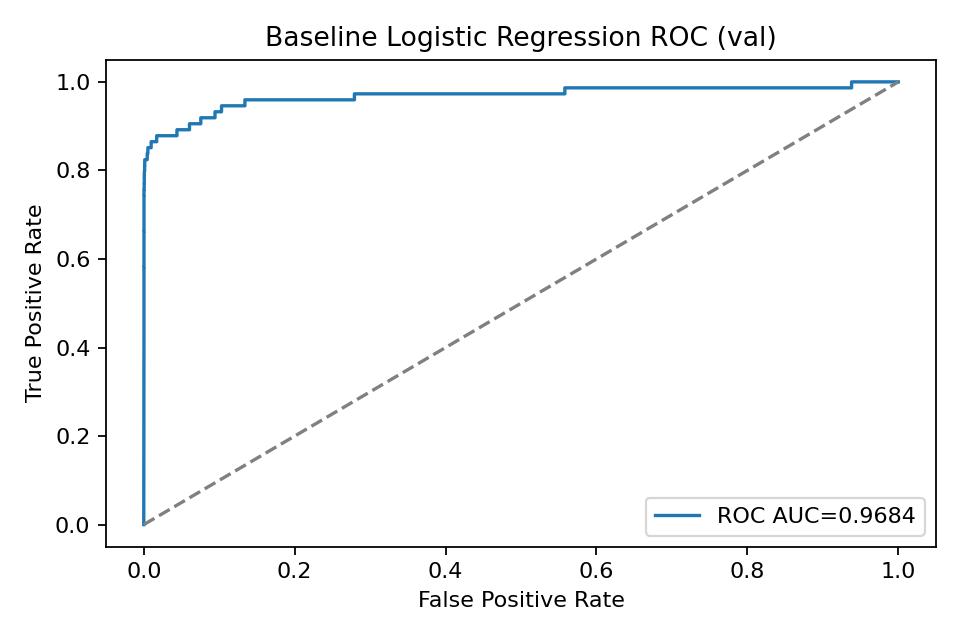
\includegraphics[width=0.8\linewidth]{../artifacts/figures/baseline_roc_curve.png}
  \caption{Baseline ROC curve. Source: \code{artifacts/figures/baseline_roc_curve.png}}
  \label{fig:base_roc}
\end{figure}
\begin{figure}[H]
  \centering
  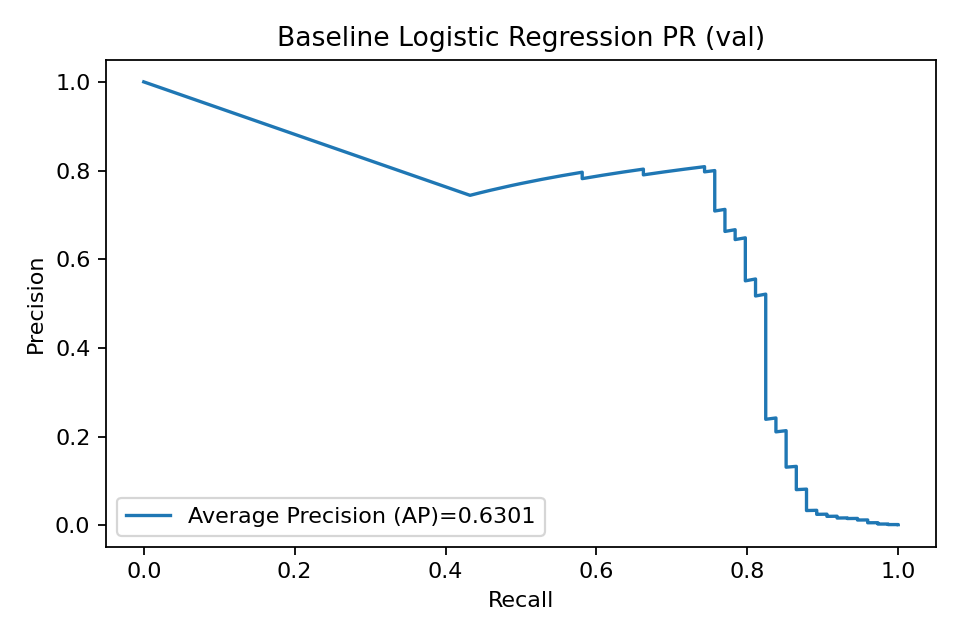
\includegraphics[width=0.8\linewidth]{../artifacts/figures/baseline_pr_curve.png}
  \caption{Baseline PR curve. Source: \code{artifacts/figures/baseline_pr_curve.png}}
  \label{fig:base_pr}
\end{figure}
\begin{figure}[H]
  \centering
  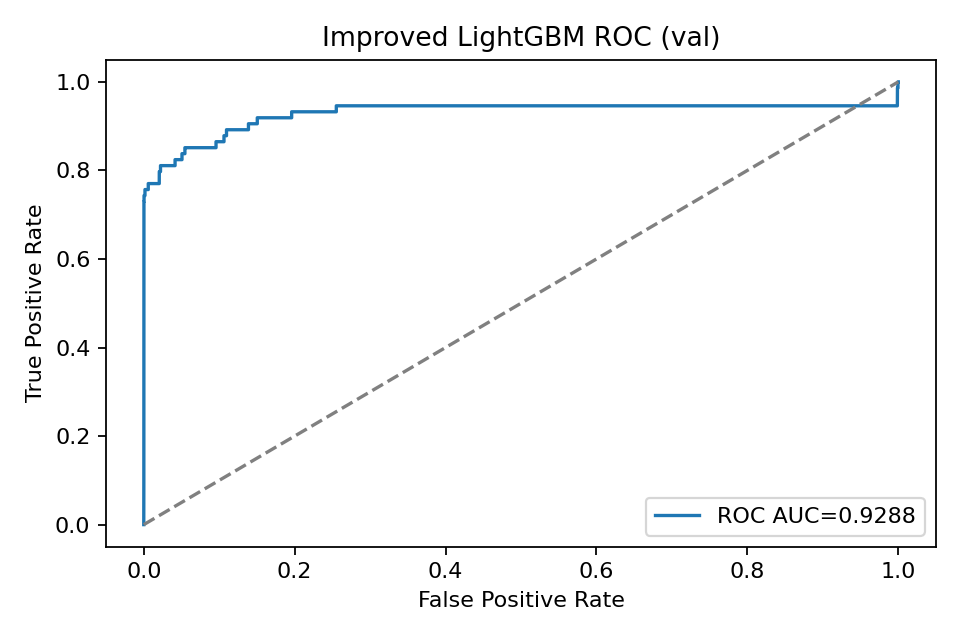
\includegraphics[width=0.8\linewidth]{../artifacts/figures/improved_roc_curve.png}
  \caption{Improved ROC curve (LightGBM). Source: \code{artifacts/figures/improved_roc_curve.png}}
  \label{fig:imp_roc}
\end{figure}
\begin{figure}[H]
  \centering
  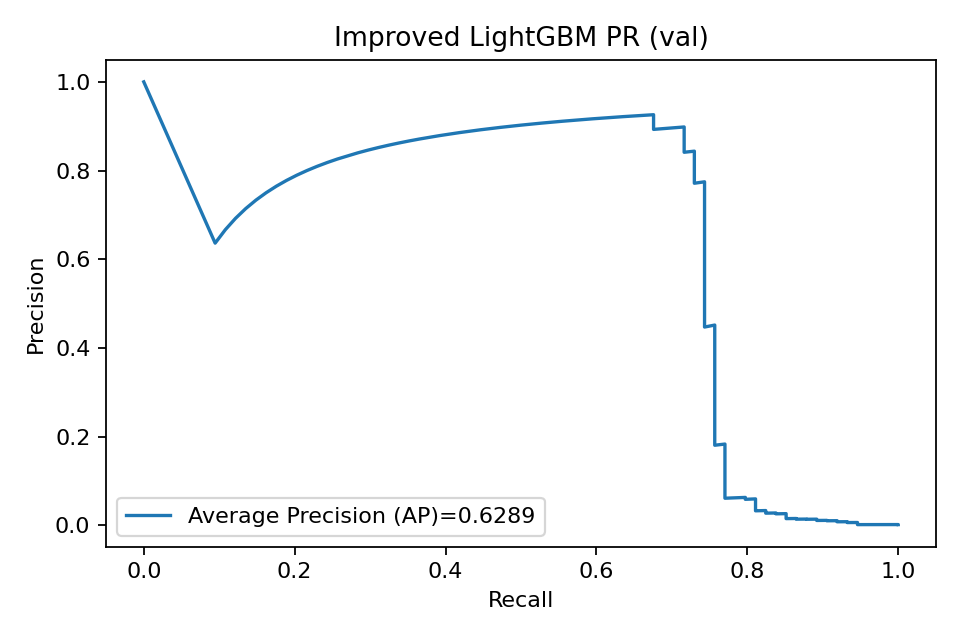
\includegraphics[width=0.8\linewidth]{../artifacts/figures/improved_pr_curve.png}
  \caption{Improved PR curve (LightGBM). Source: \code{artifacts/figures/improved_pr_curve.png}}
  \label{fig:imp_pr}
\end{figure}
\begin{figure}[H]
  \centering
  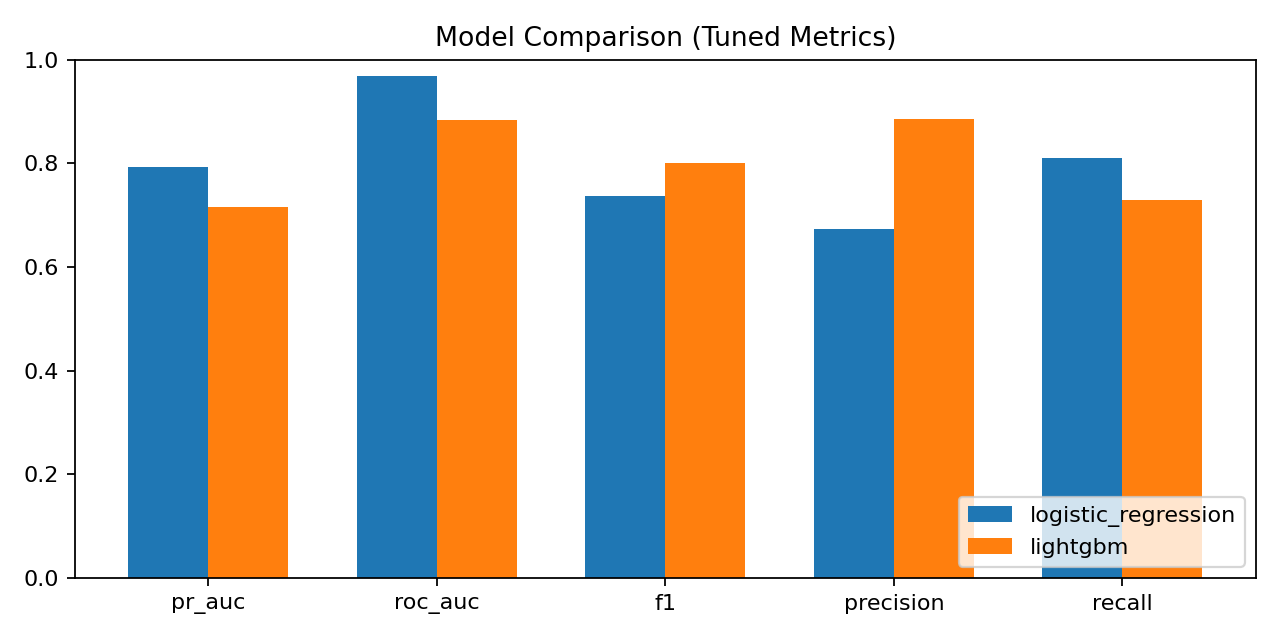
\includegraphics[width=0.9\linewidth]{../artifacts/figures/model_comparison.png}
  \caption{Model comparison (tuned metrics). Source: \code{artifacts/figures/model_comparison.png}}
  \label{fig:model_cmp}
\end{figure}

\subsection{Final deployable model diagnostics}
The selected deployable model diagnostics are shown in Figures \ref{fig:final_roc}, \ref{fig:final_pr}, and \ref{fig:final_cm}. Feature-importance evidence is provided in Figures \ref{fig:final_imp} and \ref{fig:improved_imp} for baseline and LightGBM interpretation comparison.
\begin{figure}[H]
  \centering
  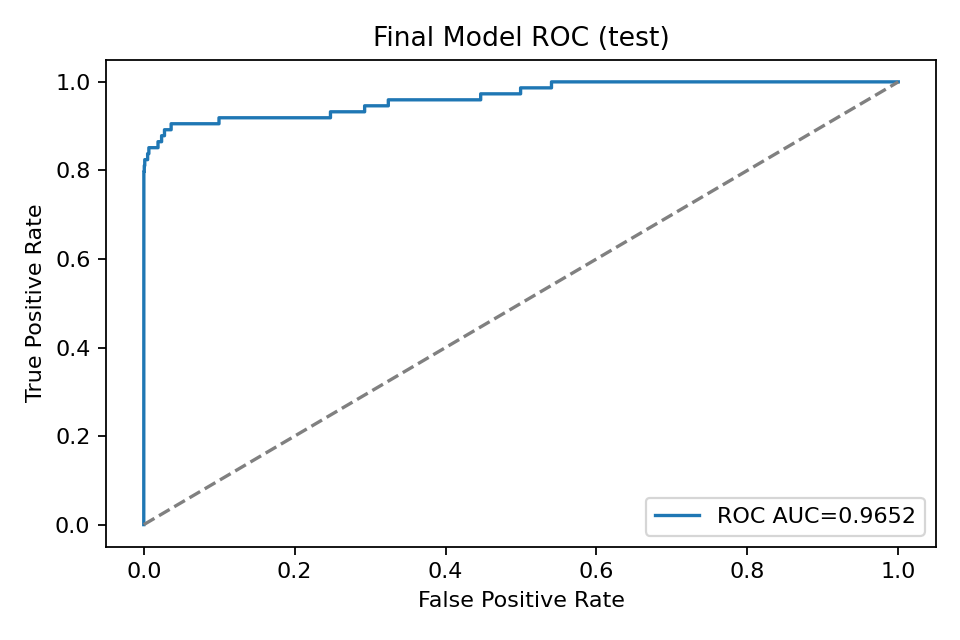
\includegraphics[width=0.82\linewidth]{../artifacts/figures/final_roc_curve.png}
  \caption{Final model ROC curve. Source: \code{artifacts/figures/final_roc_curve.png}}
  \label{fig:final_roc}
\end{figure}
\begin{figure}[H]
  \centering
  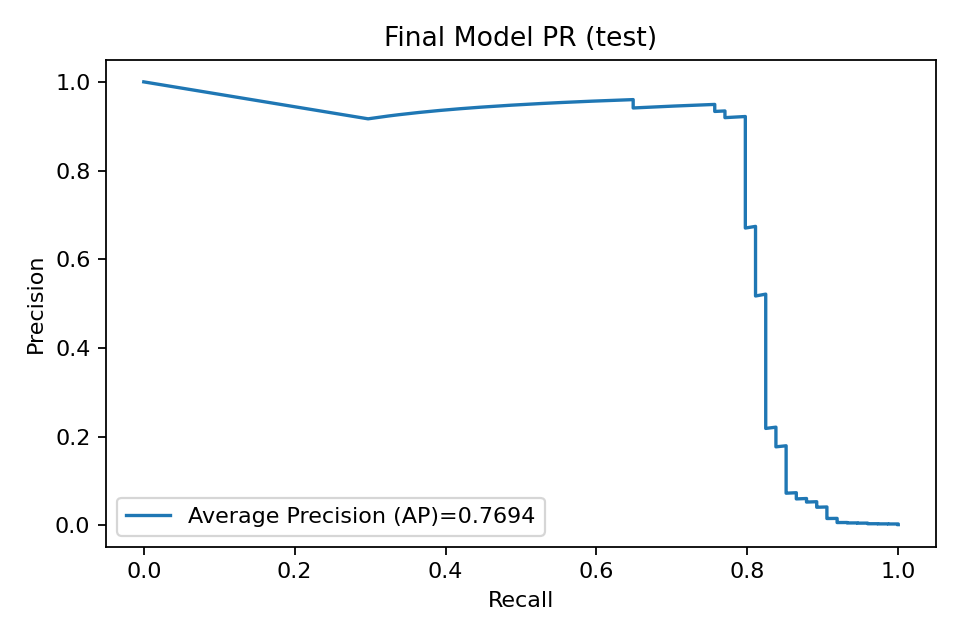
\includegraphics[width=0.82\linewidth]{../artifacts/figures/final_pr_curve.png}
  \caption{Final model PR curve. Source: \code{artifacts/figures/final_pr_curve.png}}
  \label{fig:final_pr}
\end{figure}
\begin{figure}[H]
  \centering
  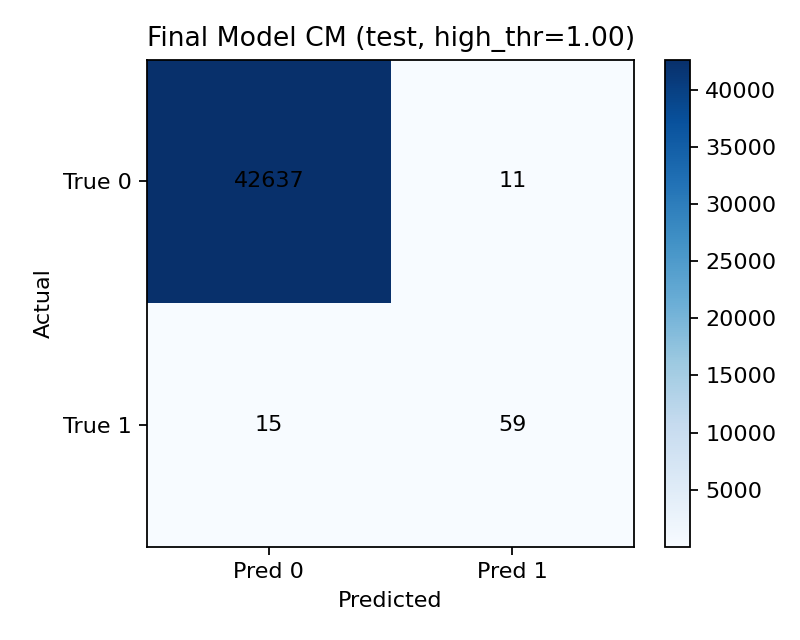
\includegraphics[width=0.72\linewidth]{../artifacts/figures/final_confusion_matrix.png}
  \caption{Final model confusion matrix. Source: \code{artifacts/figures/final_confusion_matrix.png}}
  \label{fig:final_cm}
\end{figure}
\begin{figure}[H]
  \centering
  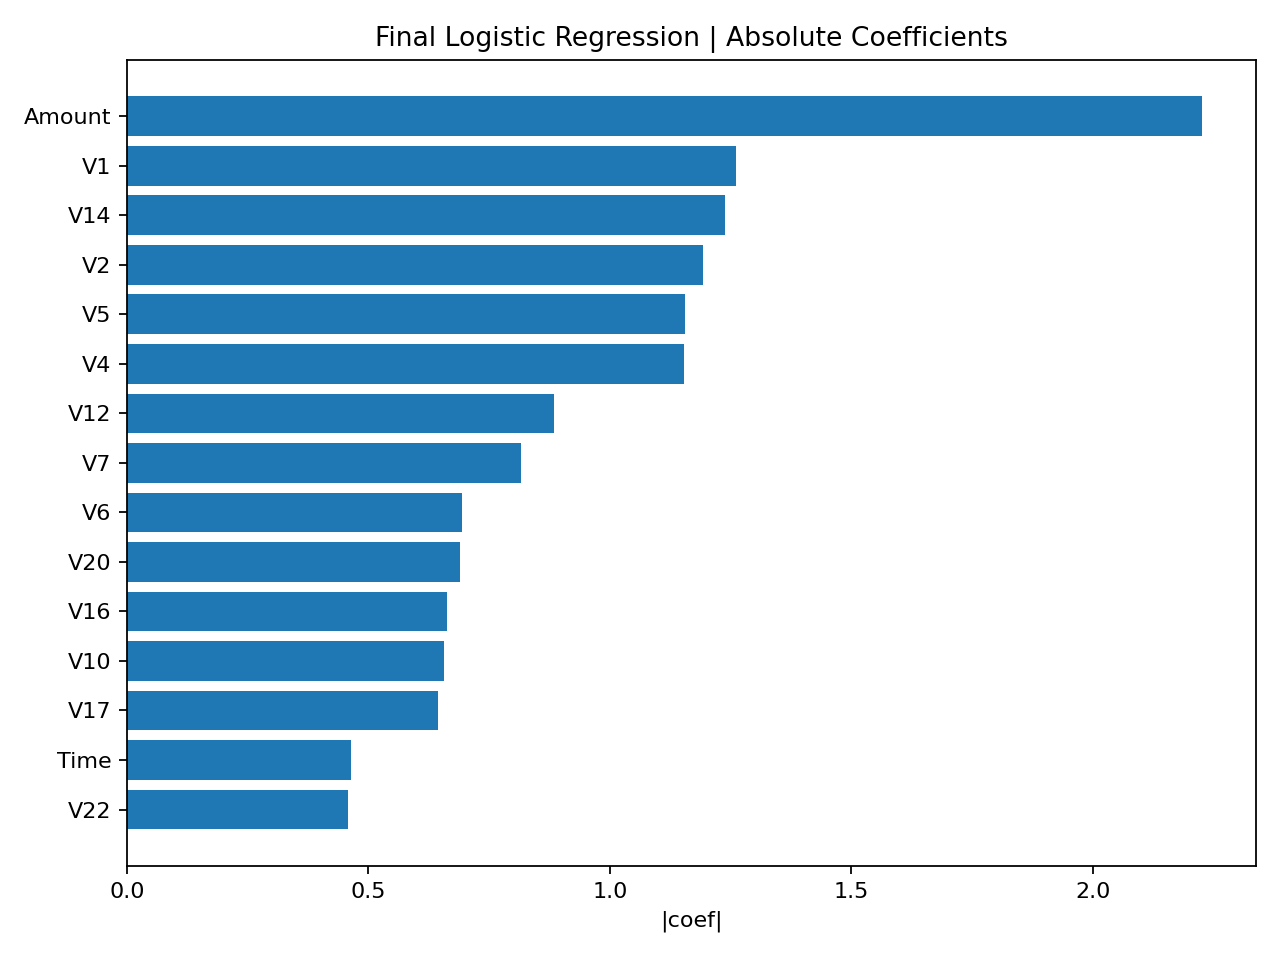
\includegraphics[width=0.85\linewidth]{../artifacts/figures/final_feature_importance.png}
  \caption{Final model feature importance. Source: \code{artifacts/figures/final_feature_importance.png}}
  \label{fig:final_imp}
\end{figure}
\begin{figure}[H]
  \centering
  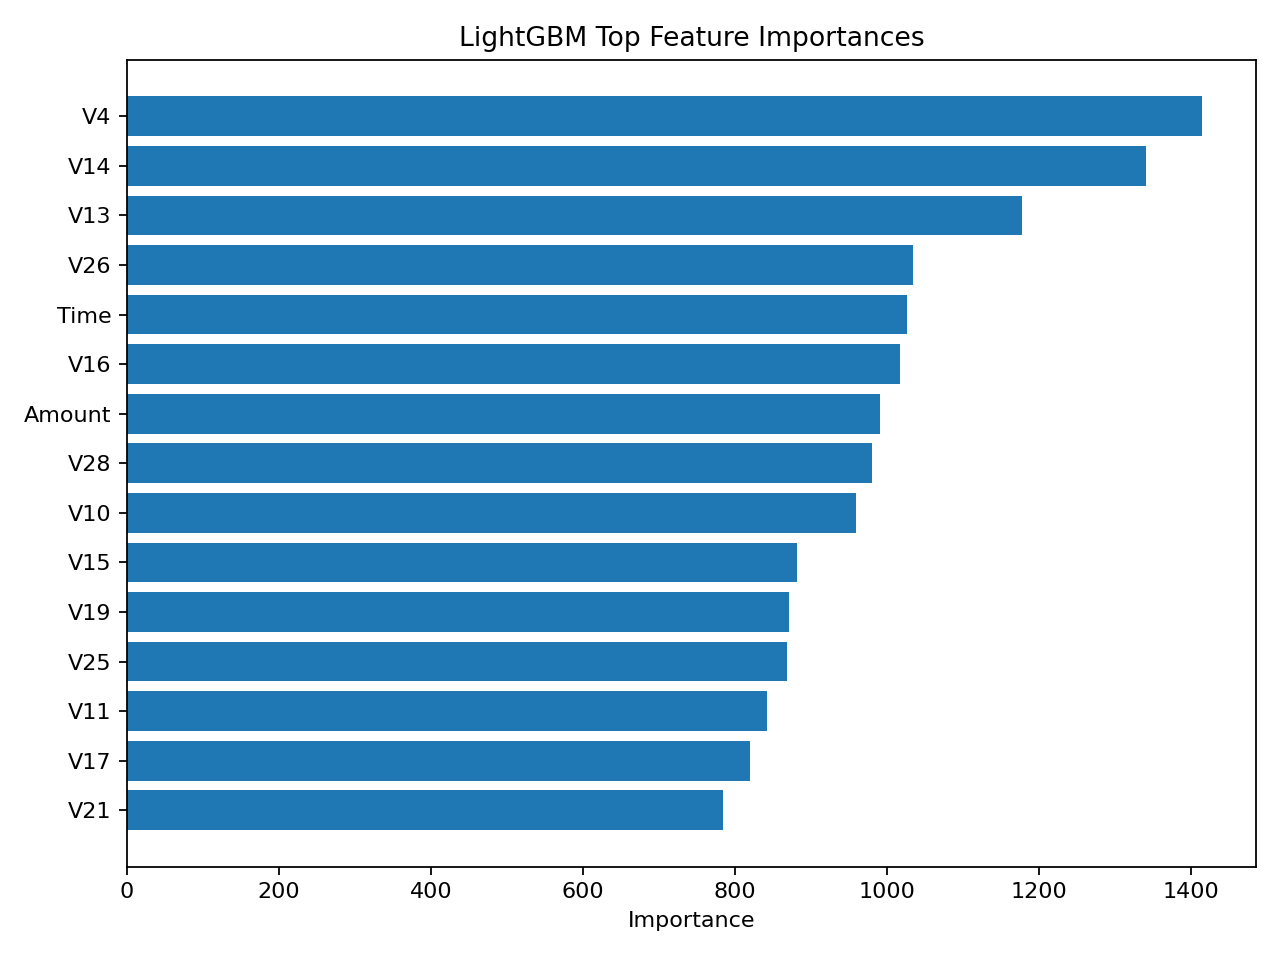
\includegraphics[width=0.85\linewidth]{../artifacts/figures/improved_feature_importance.png}
  \caption{Improved model feature importance (LightGBM). Source: \code{artifacts/figures/improved_feature_importance.png}}
  \label{fig:improved_imp}
\end{figure}

\section{Threshold Tuning}
\subsection{How it works (evidence)}
In \code{src/pipelines/run_model_workflow.py}, the system:
\begin{itemize}
  \item sweeps thresholds from 0.01 to 0.99 on validation scores
  \item selects the threshold that maximizes F1 on validation
  \item evaluates the tuned threshold on the test split and records it in model metadata
\end{itemize}
Threshold sweep tables: \code{artifacts/benchmarks/baseline_threshold_tuning.csv}, \code{artifacts/benchmarks/improved_threshold_tuning.csv}, plus overlay comparison \code{artifacts/benchmarks/threshold_comparison_table.csv}.

\subsection{Numeric tuning evidence (from validation sweeps)}
From the sweep tables (best-by-F1 on validation):
\begin{itemize}
  \item Baseline best validation threshold: 0.99 (validation F1=0.6629)
  \item Improved best validation threshold: 0.84 (validation F1=0.7970)
\end{itemize}

\subsection{Embedded threshold figures}
Threshold behavior and cross-model operating-point differences are illustrated in Figures \ref{fig:base_thr}, \ref{fig:imp_thr}, and \ref{fig:thr_cmp}.
\begin{figure}[H]
  \centering
  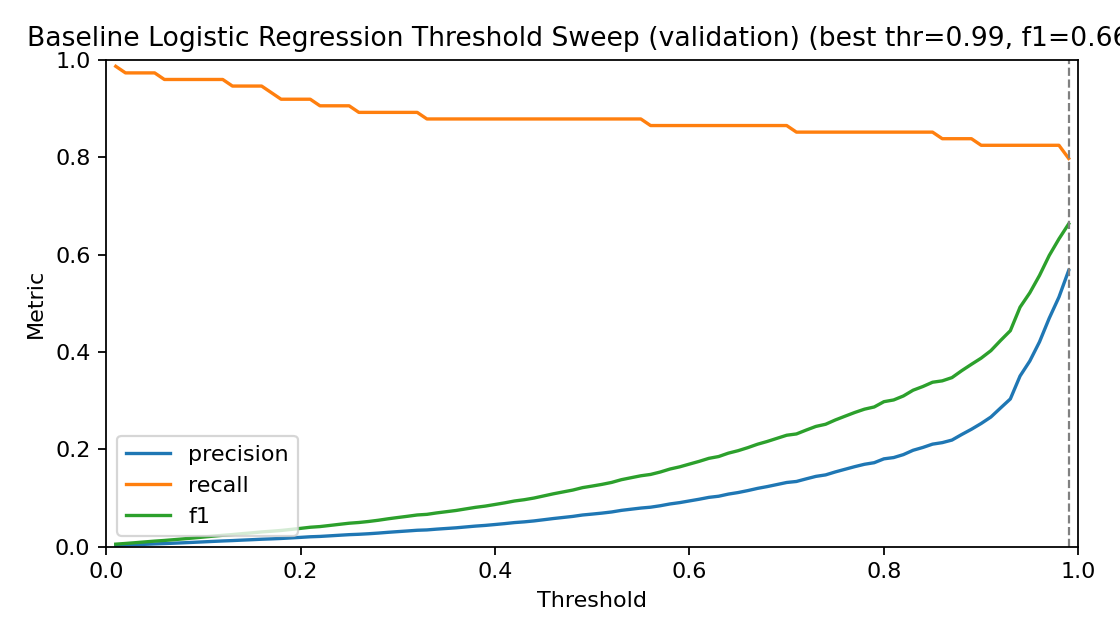
\includegraphics[width=0.9\linewidth]{../artifacts/figures/baseline_threshold_sweep.png}
  \caption{Baseline threshold sweep. Source: \code{artifacts/figures/baseline_threshold_sweep.png}}
  \label{fig:base_thr}
\end{figure}
\begin{figure}[H]
  \centering
  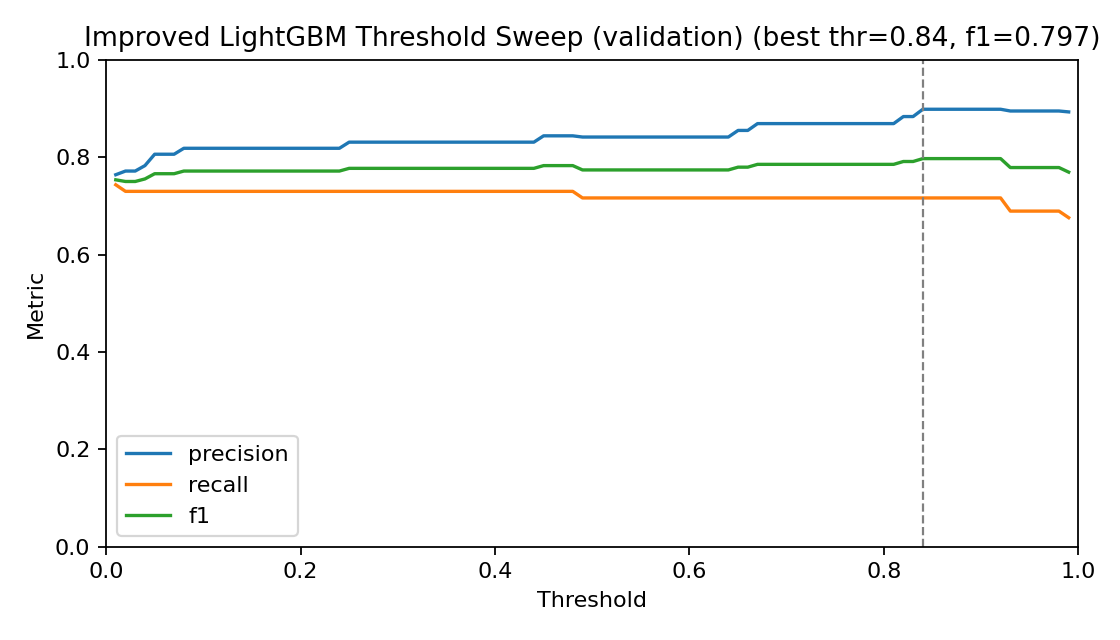
\includegraphics[width=0.9\linewidth]{../artifacts/figures/improved_threshold_sweep.png}
  \caption{Improved threshold sweep. Source: \code{artifacts/figures/improved_threshold_sweep.png}}
  \label{fig:imp_thr}
\end{figure}
\begin{figure}[H]
  \centering
  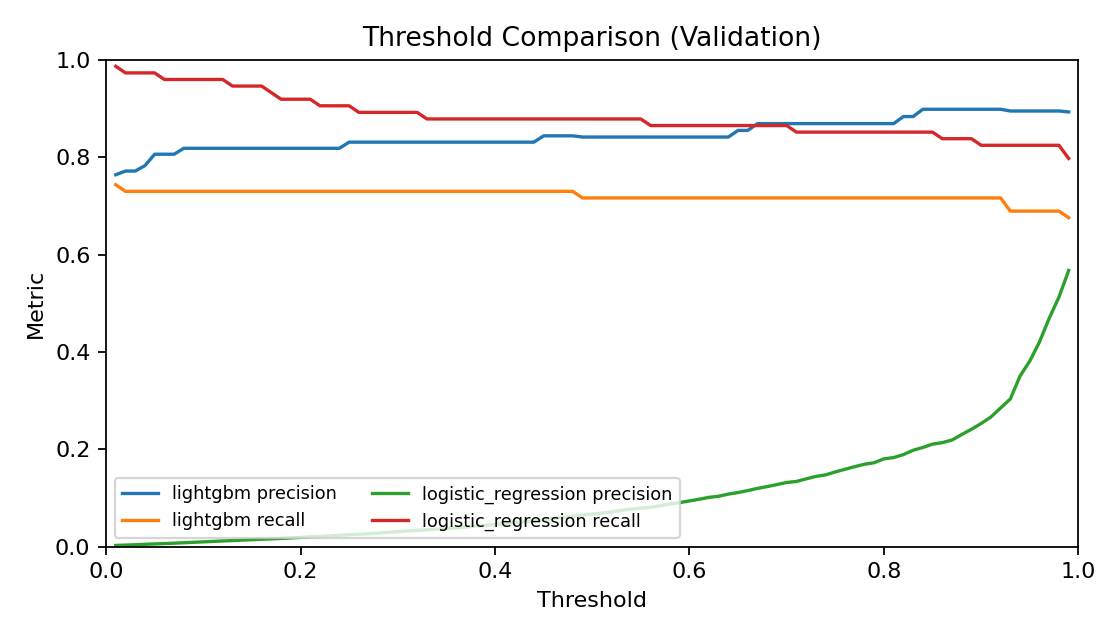
\includegraphics[width=0.9\linewidth]{../artifacts/figures/threshold_comparison.png}
  \caption{Threshold comparison overlay (F1 curves). Source: \code{artifacts/figures/threshold_comparison.png}}
  \label{fig:thr_cmp}
\end{figure}

\section{Model Explainability (SHAP)}
\subsection{What is implemented (evidence)}
\code{src/pipelines/run_model_workflow.py} computes SHAP values for the LightGBM candidate model using \code{shap.TreeExplainer}, exporting:
\begin{itemize}
  \item SHAP summary plot: \code{artifacts/figures/shap_summary.png}
  \item SHAP importance table: \code{artifacts/benchmarks/shap_importance_table.csv}
\end{itemize}
\textbf{Constraint (no assumption):} SHAP is generated for LightGBM even though the selected deployable model in this artifact set is Logistic Regression.

\begin{figure}[H]
  \centering
  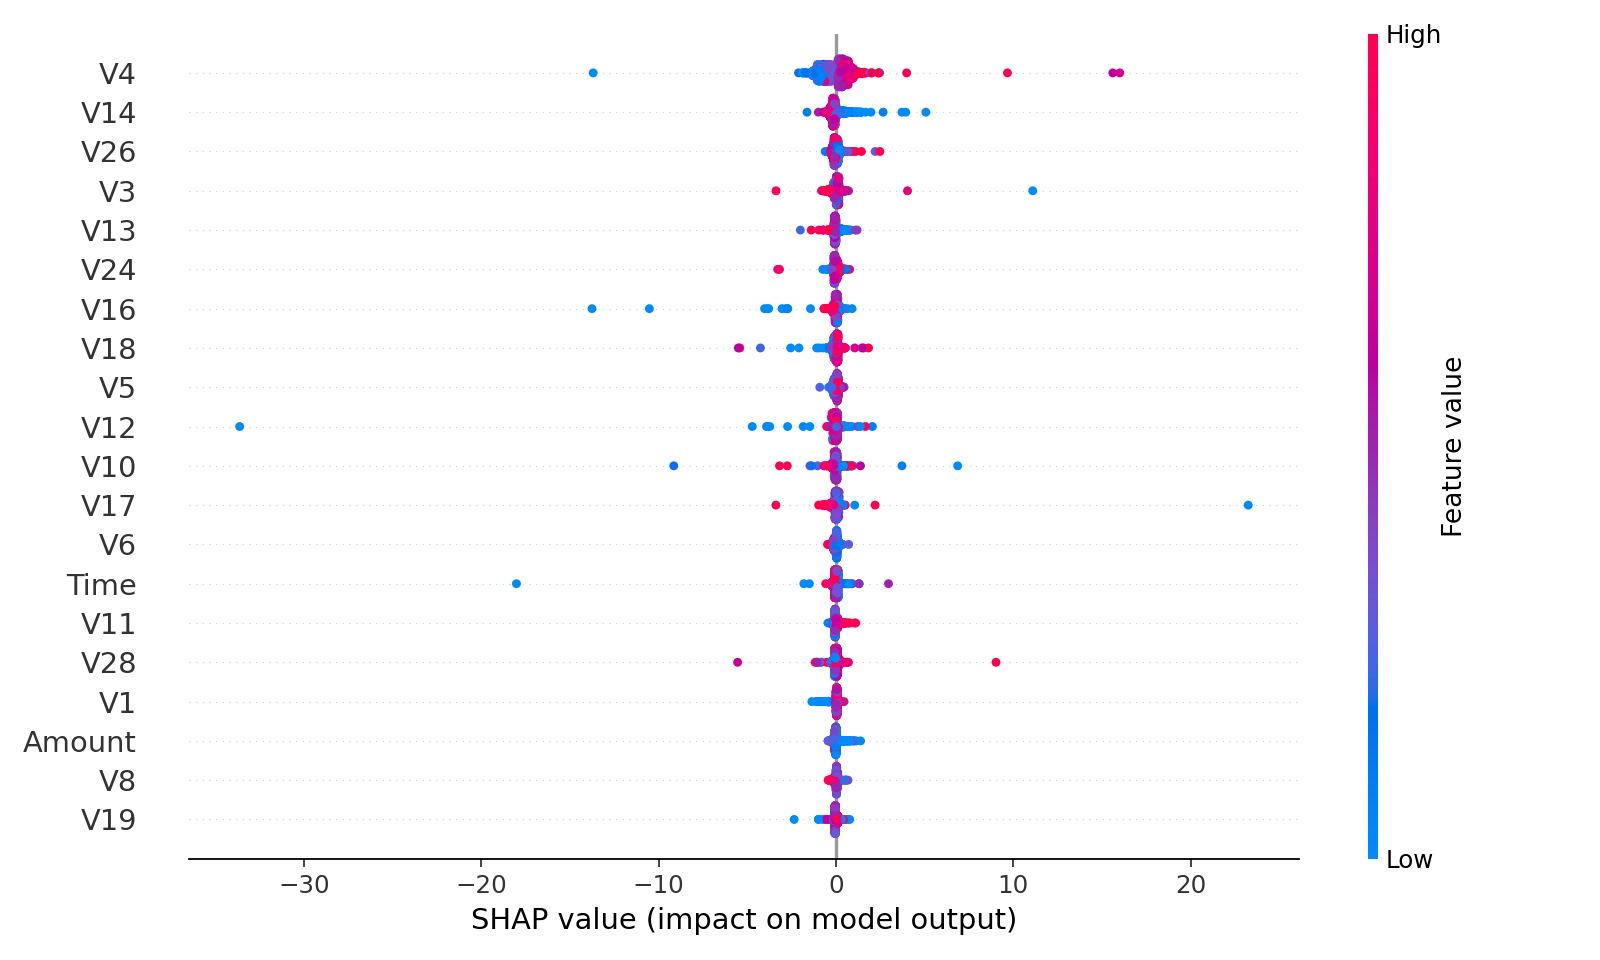
\includegraphics[width=0.95\linewidth]{../artifacts/figures/shap_summary.png}
  \caption{SHAP summary plot (LightGBM). Source: \code{artifacts/figures/shap_summary.png}}
  \label{fig:shap_summary}
\end{figure}

\section{System Architecture (E2E flow)}
\subsection{Architecture diagram (embedded)}
This diagram reflects the implemented structure described in \code{ARCHITECTURE.md} and wired by \code{deployment/docker-compose.yml}.

\begin{figure}[H]
  \centering
  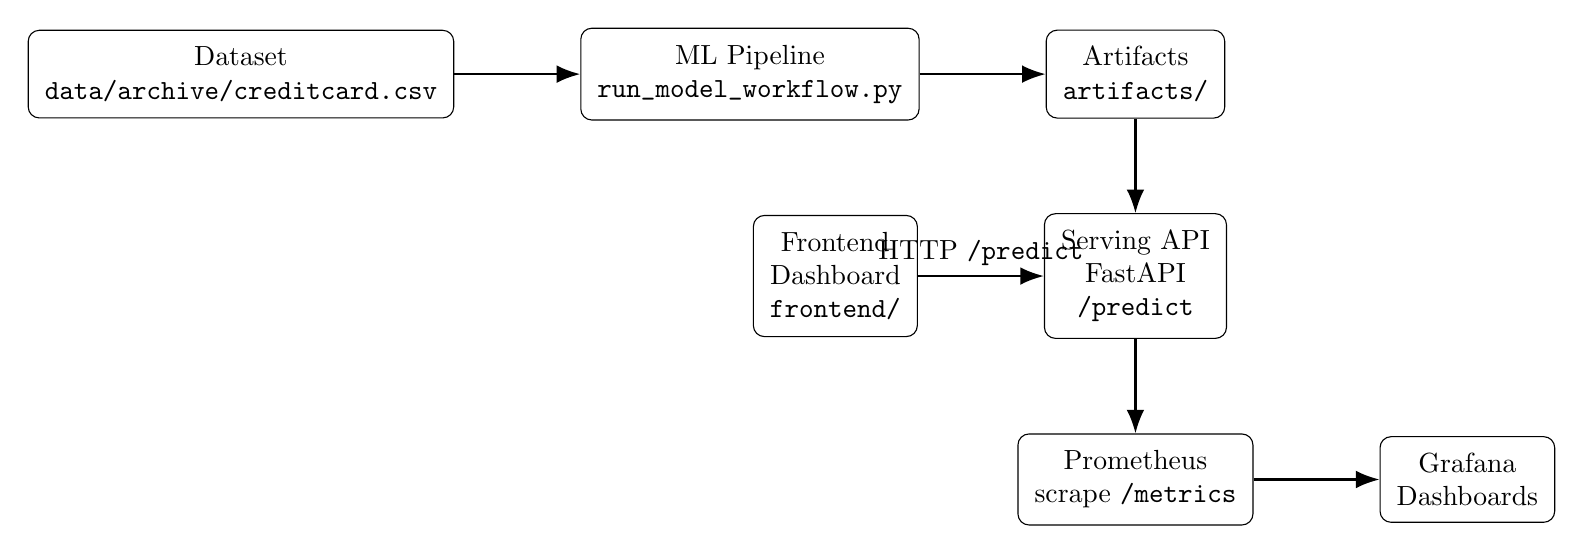
\begin{tikzpicture}[
    node/.style={draw, rounded corners, align=center, inner sep=6pt},
    arrow/.style={-{Latex[length=3mm]}, thick}
  ]
    \node[node] (ds) {Dataset\\\code{data/archive/creditcard.csv}};
    \node[node, right=1.6cm of ds] (pipe) {ML Pipeline\\\code{run_model_workflow.py}};
    \node[node, right=1.6cm of pipe] (art) {Artifacts\\\code{artifacts/}};

    \node[node, below=1.2cm of art] (api) {Serving API\\FastAPI\\\code{/predict}};
    \node[node, left=1.6cm of api] (fe) {Frontend\\Dashboard\\\code{frontend/}};

    \node[node, below=1.2cm of api] (prom) {Prometheus\\scrape \code{/metrics}};
    \node[node, right=1.6cm of prom] (graf) {Grafana\\Dashboards};

    \draw[arrow] (ds) -- (pipe);
    \draw[arrow] (pipe) -- (art);
    \draw[arrow] (art) -- (api);
    \draw[arrow] (fe) -- node[above, sloped]{HTTP \code{/predict}} (api);
    \draw[arrow] (api) -- (prom);
    \draw[arrow] (prom) -- (graf);
  \end{tikzpicture}
  \caption{End-to-end architecture (implementation-aligned).}
  \label{fig:e2e_arch}
\end{figure}

\subsection{Contract boundary (evidence)}
The feature contract for the Kaggle model is 30 floats ordered as \code{[Time, V1..V28, Amount]}:
\begin{itemize}
  \item stored in \code{artifacts/models/model_info.json} as \code{feature_columns}
  \item enforced by API length checks in \code{src/api/main.py}
  \item enforced by frontend client checks in \code{frontend/api-client.js}
\end{itemize}

\section{API Design}
\subsection{Endpoints (implemented)}
Implemented in \code{src/api/main.py}:
\begin{itemize}
  \item \code{GET /health} (model loaded status + metadata)
  \item \code{POST /predict} (fraud probability + threshold-based label)
  \item \code{GET /metrics} (Prometheus exposition)
  \item \code{GET /dataset/samples} (dataset-backed sampling; mixed/fraud/legit)
  \item Additional: \code{/features/schema}, \code{/features/random}
\end{itemize}

\subsection{Schema evidence}
Request and response shapes are defined in \code{src/api/schemas.py}. \code{/predict} returns:
\code{request_id}, \code{risk_score}, \code{risk_tier}/\code{action}, \code{threshold_review}/\code{threshold_high}, \code{model_version}, plus optional metadata.

\subsection{Runtime examples}
\textbf{Status:} \statusunverified{} (API was not launched in this report generation environment).  
To capture real JSON evidence, run the repo's verification harness \code{verify_system.py} after starting the API, or use the command sequence in \code{FINAL_E2E_REPORT.md}.

\section{Frontend System (UI/UX)}
\subsection{Dashboard layout (evidence)}
From \code{frontend/index.html}, the dashboard includes:
\begin{itemize}
  \item Connection pill + model metadata (version, thresholds review/high, expected features)
  \item Control panel (API URL, mode, speed, start/stop/reset)
  \item KPIs (counts, rates, avg risk score, last latency)
  \item Alert panel (Review/High)
  \item Probability-over-time chart (canvas)
  \item Append-only transaction feed table
\end{itemize}

\subsection{Streaming and alerting logic (evidence)}
From \code{frontend/app.js}:
\begin{itemize}
  \item Streams transactions at 0.5s / 1s / 2s intervals, calling \code{POST /predict}
  \item Risk tiers: LOW if score \(< \) \code{threshold\_review}; REVIEW if between thresholds; HIGH if score \( \ge \) \code{threshold\_high}
  \item Stops stream after 4 consecutive errors (demo stability)
\end{itemize}
Real sample pool is fetched from the backend dataset endpoint (\code{GET /dataset/samples}) using production-like sampling, with rare fraud spikes for demo visibility.

\subsection{Embedded frontend screenshot}
\begin{figure}[H]
  \centering
  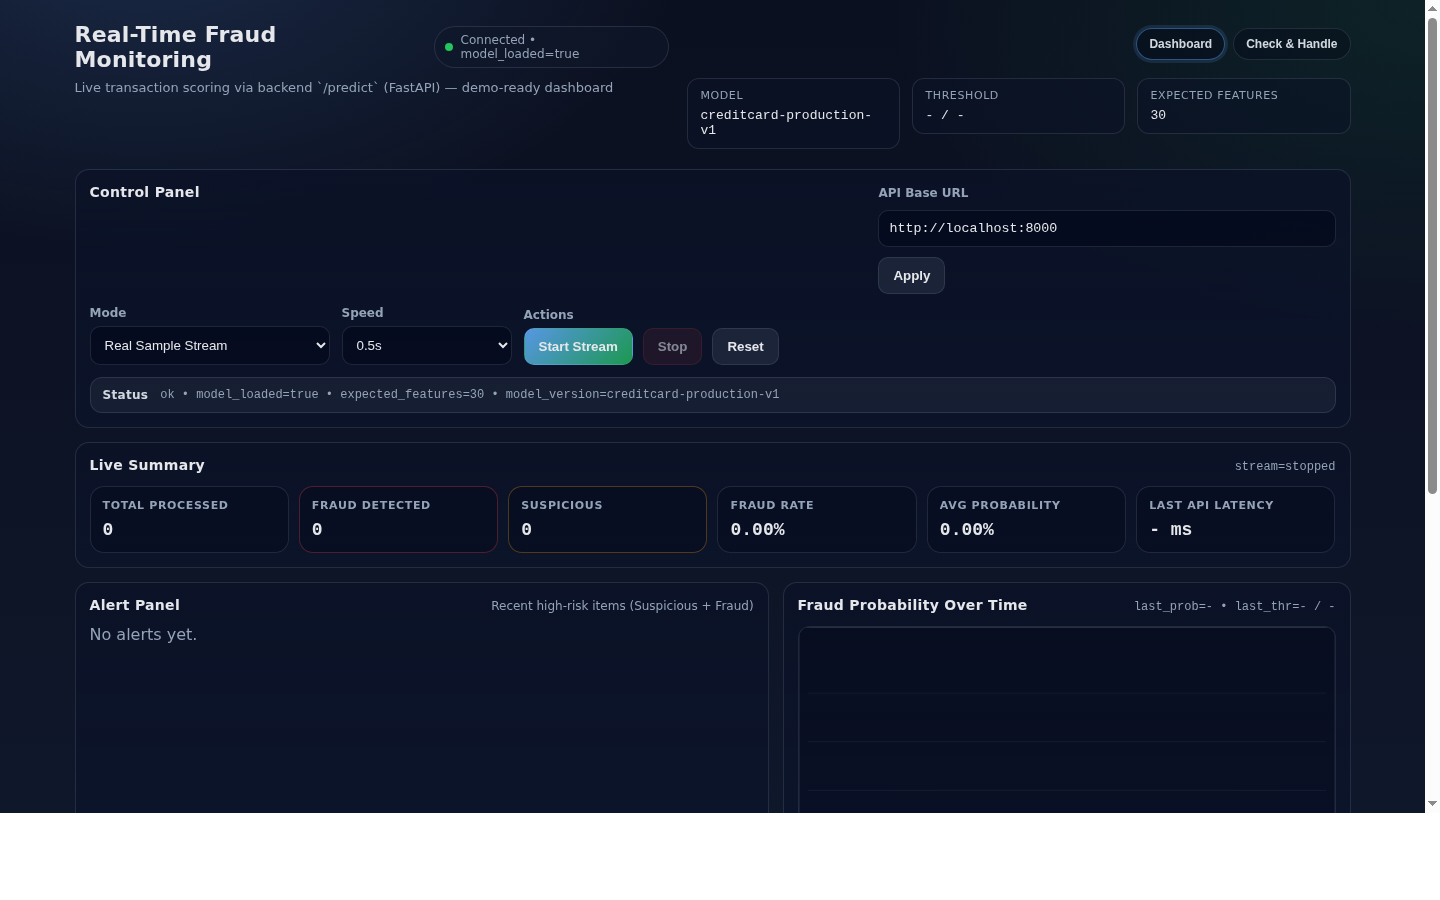
\includegraphics[width=0.95\linewidth]{../artifacts/figures/frontend_dashboard_live.png}
  \caption{Frontend dashboard screenshot (connected to backend). Source: \code{artifacts/figures/frontend_dashboard_live.png}.}
  \label{fig:frontend_live}
\end{figure}
\begin{figure}[H]
  \centering
  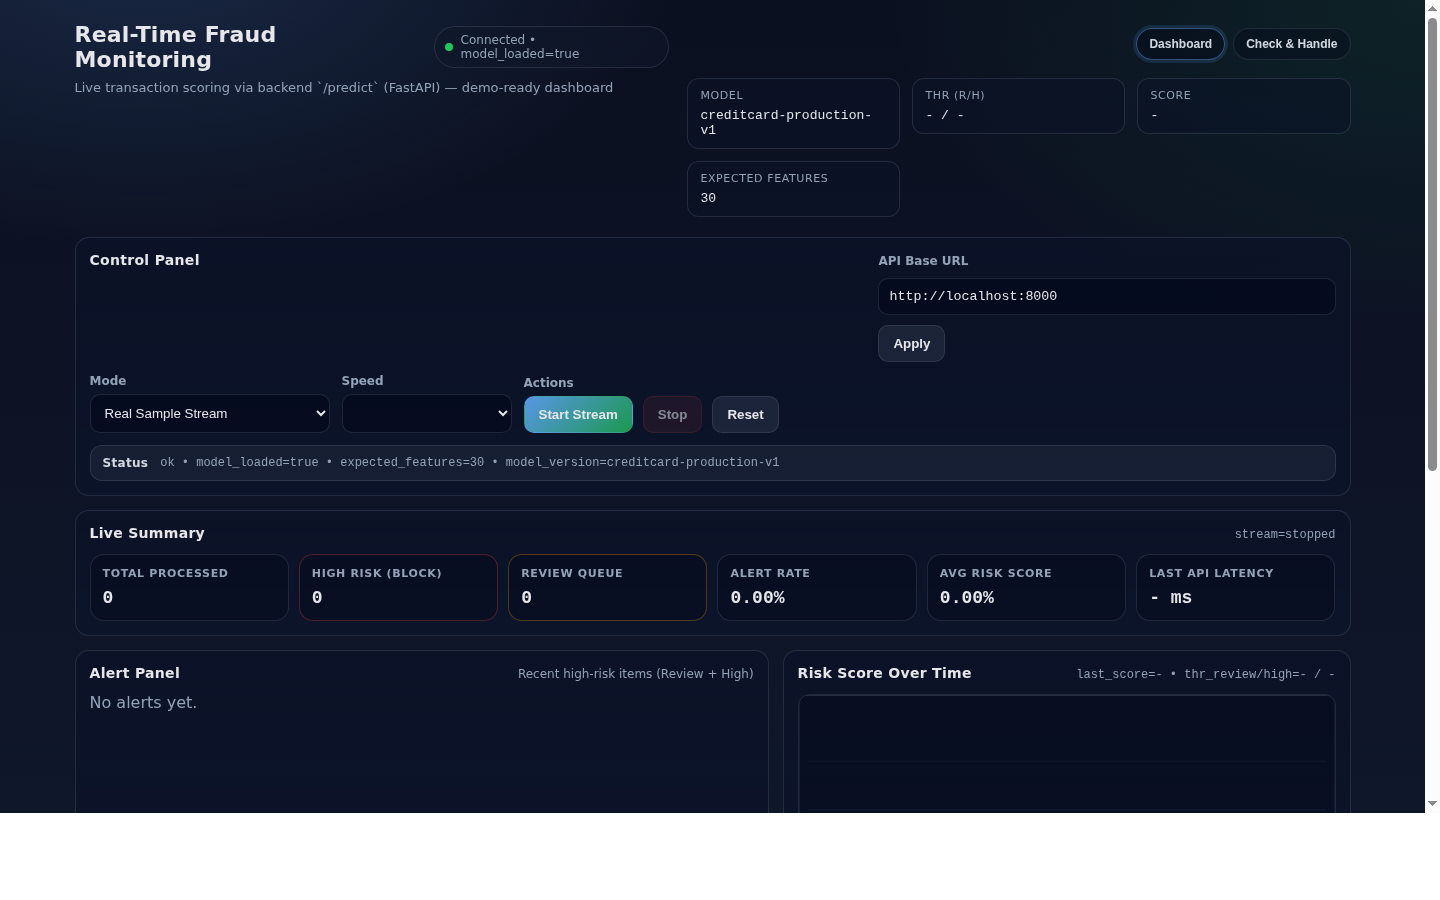
\includegraphics[width=0.95\linewidth]{../artifacts/figures/frontend_dashboard_streaming.png}
  \caption{Frontend streaming mode screenshot. Source: \code{artifacts/figures/frontend_dashboard_streaming.png}.}
  \label{fig:frontend_stream}
\end{figure}
\textbf{Note:} Headless screenshot capture does not reliably wait for asynchronous streaming updates; the screenshot shows a connected dashboard ready to stream. A live ``stream running'' screenshot is a TODO for manual capture during demo rehearsal.

\section{API Behavior Examples (Captured Outputs)}
\subsection{How these examples were captured}
To avoid network namespace issues in automated runs, API examples were captured by calling the FastAPI ASGI app directly (with lifespan startup) using the repo's ASGI test harness (\code{tests/integration/asgi_client.py}). The captured outputs are saved in:
\begin{itemize}
  \item \code{artifacts/reports/api_example_health.json}
  \item \code{artifacts/reports/api_example_dataset_samples.json}
  \item \code{artifacts/reports/api_example_predict.json}
  \item \code{artifacts/reports/api_example_metrics.txt}
\end{itemize}

\subsection{Example: \code{GET /health}}
\VerbatimInput[fontsize=\small,frame=single,breaklines=true]{\detokenize{../artifacts/reports/api_example_health.json}}

\subsection{Example: \code{GET /dataset/samples?n=1\&strategy=legit}}
\VerbatimInput[fontsize=\small,frame=single,breaklines=true]{\detokenize{../artifacts/reports/api_example_dataset_samples.json}}

\subsection{Example: \code{POST /predict}}
\VerbatimInput[fontsize=\small,frame=single,breaklines=true]{\detokenize{../artifacts/reports/api_example_predict.json}}


\section{Monitoring \& Alerts}
\subsection{Metrics emitted (evidence)}
From \code{src/monitoring/metrics.py}, the API emits:
\begin{itemize}
  \item \code{api_requests_total\{endpoint,method,http_status\}}
  \item \code{api_request_latency_seconds} histogram (p95 computed by Prometheus)
  \item \code{fraud_predictions_total\{label\}}
  \item \code{fraud_scores_sum} and \code{fraud_scores_count} (avg score)
\end{itemize}

\subsection{Prometheus scrape and rules (evidence)}
Scrape config: \code{deployment/prometheus/prometheus.yml}. Alert rules: \code{deployment/prometheus/alerts.yml}, including:
high 5xx error rate, high p95 latency, and prediction-rate anomaly alerts.

\subsection{Grafana dashboard (evidence)}
Dashboard JSON: \code{deployment/grafana/dashboards/fraud_api.json}.  
\begin{figure}[H]
  \centering
  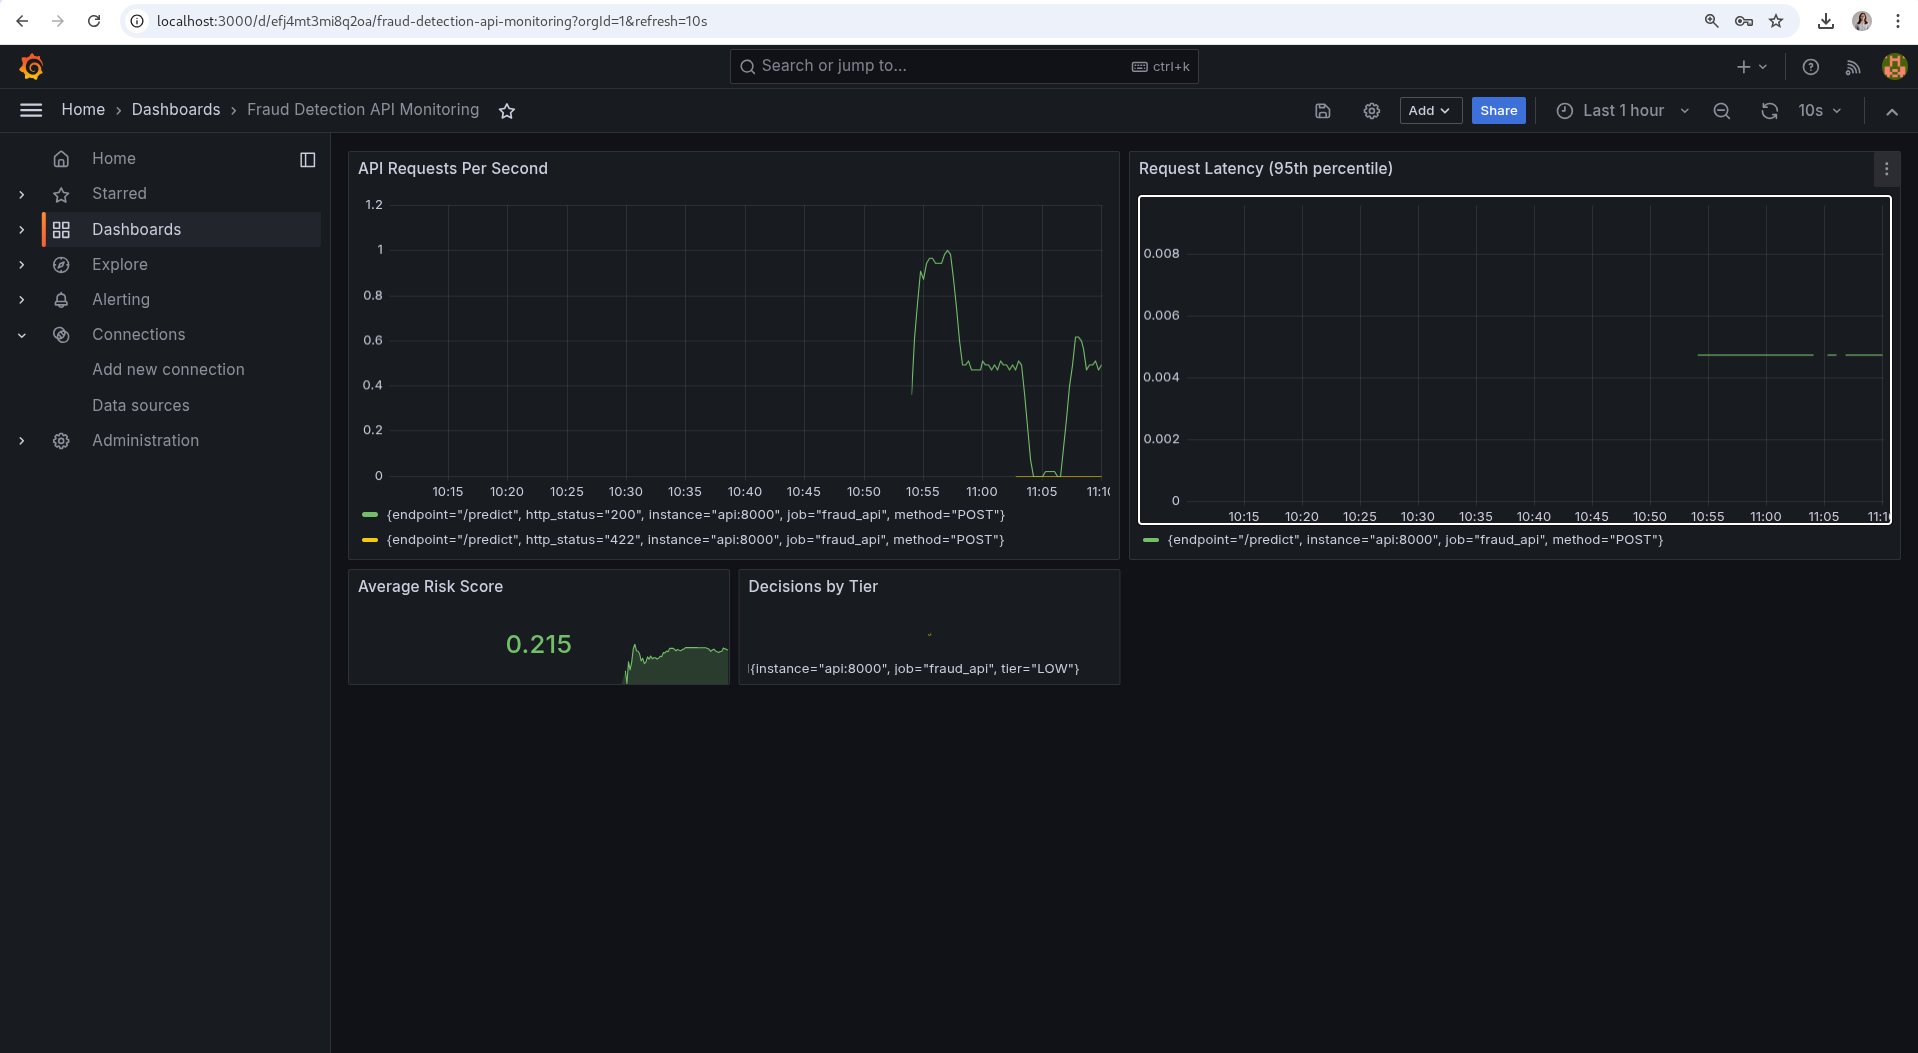
\includegraphics[width=0.92\linewidth]{../artifacts/deploys/Grafana-dashboard.png}
  \caption{Grafana dashboard screenshot. Source: \code{artifacts/deploys/Grafana-dashboard.png}}
  \label{fig:grafana_dash}
\end{figure}
\begin{figure}[H]
  \centering
  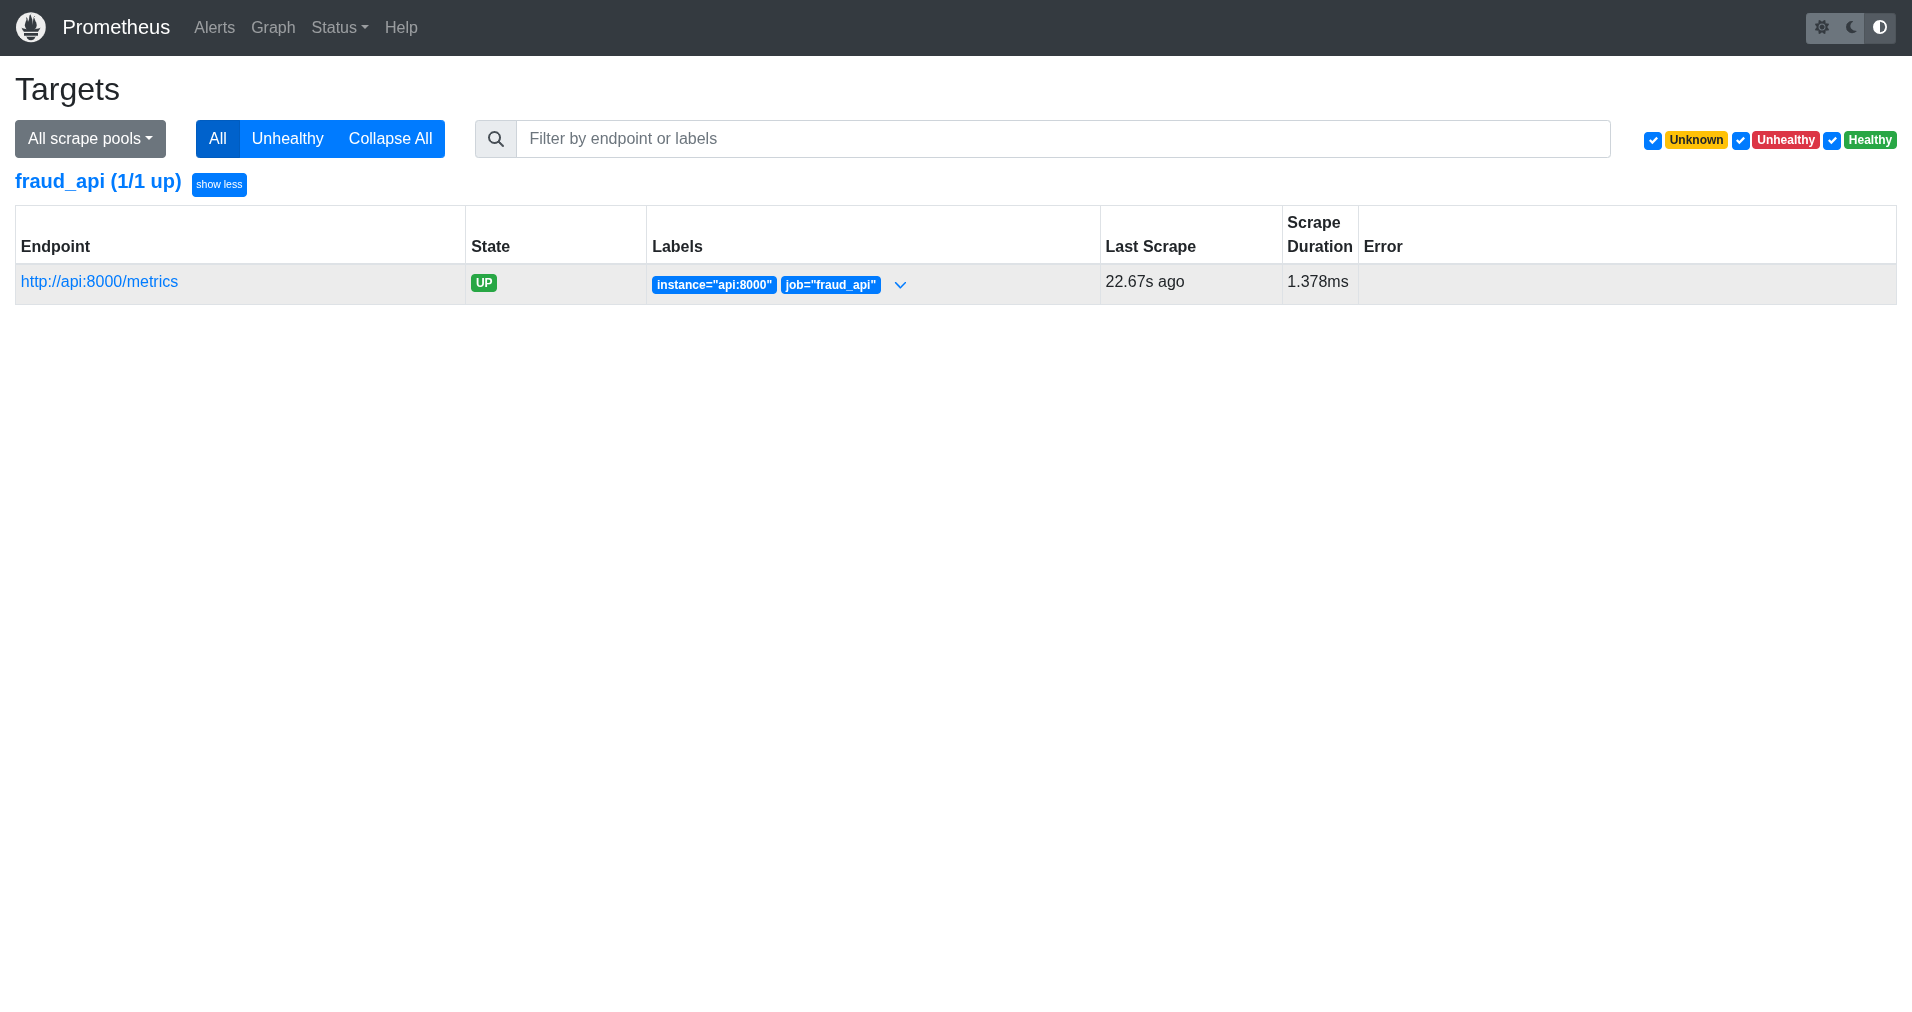
\includegraphics[width=0.92\linewidth]{../artifacts/deploys/Prometheus-targets.png}
  \caption{Prometheus targets screenshot. Source: \code{artifacts/deploys/Prometheus-targets.png}}
  \label{fig:prom_targets}
\end{figure}
\begin{figure}[H]
  \centering
  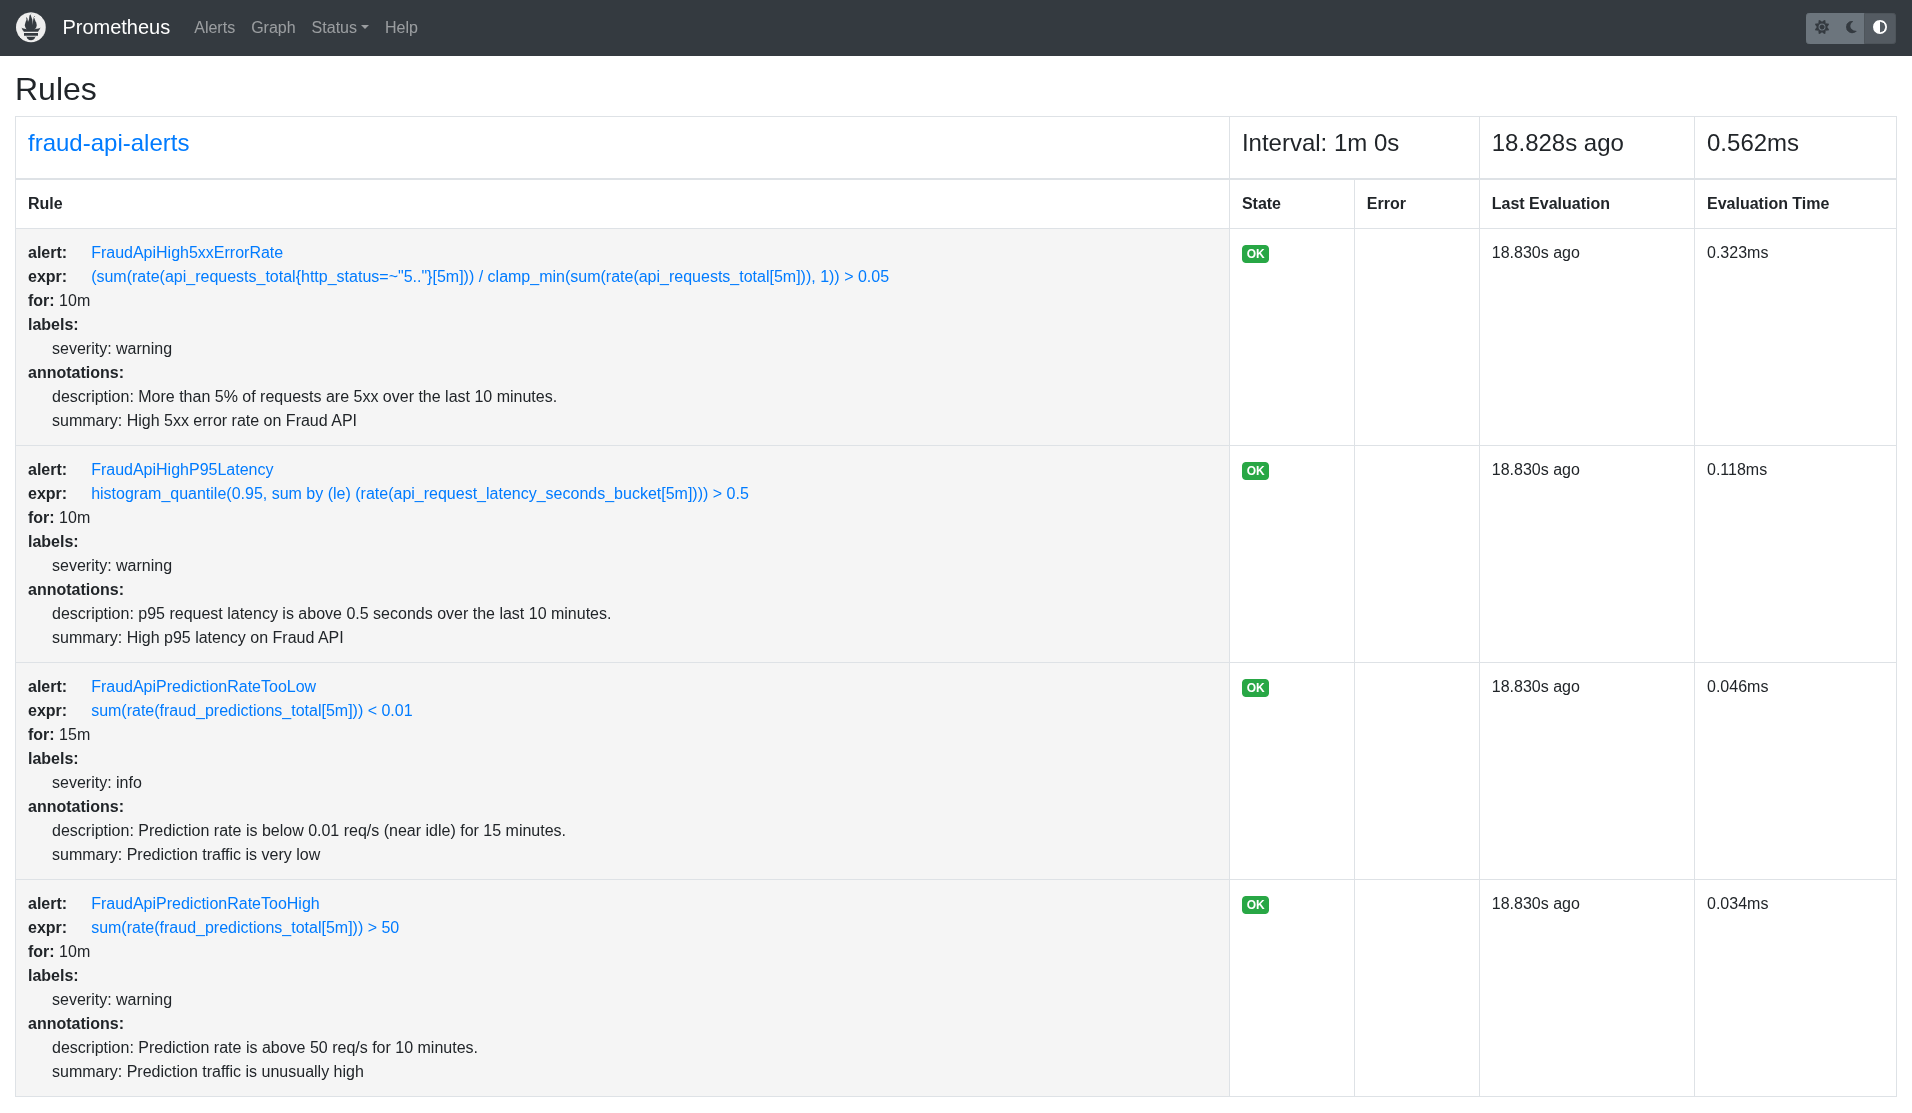
\includegraphics[width=0.92\linewidth]{../artifacts/deploys/Prometheus-rules.png}
  \caption{Prometheus alert rules screenshot. Source: \code{artifacts/deploys/Prometheus-rules.png}}
  \label{fig:prom_rules}
\end{figure}

\section{Deployment}
\subsection{Docker Compose stack (evidence)}
From \code{deployment/docker-compose.yml}, services include:
API (8000), frontend (8080), MLflow (5000), Prometheus (9090), Grafana (3000).
\begin{figure}[H]
  \centering
  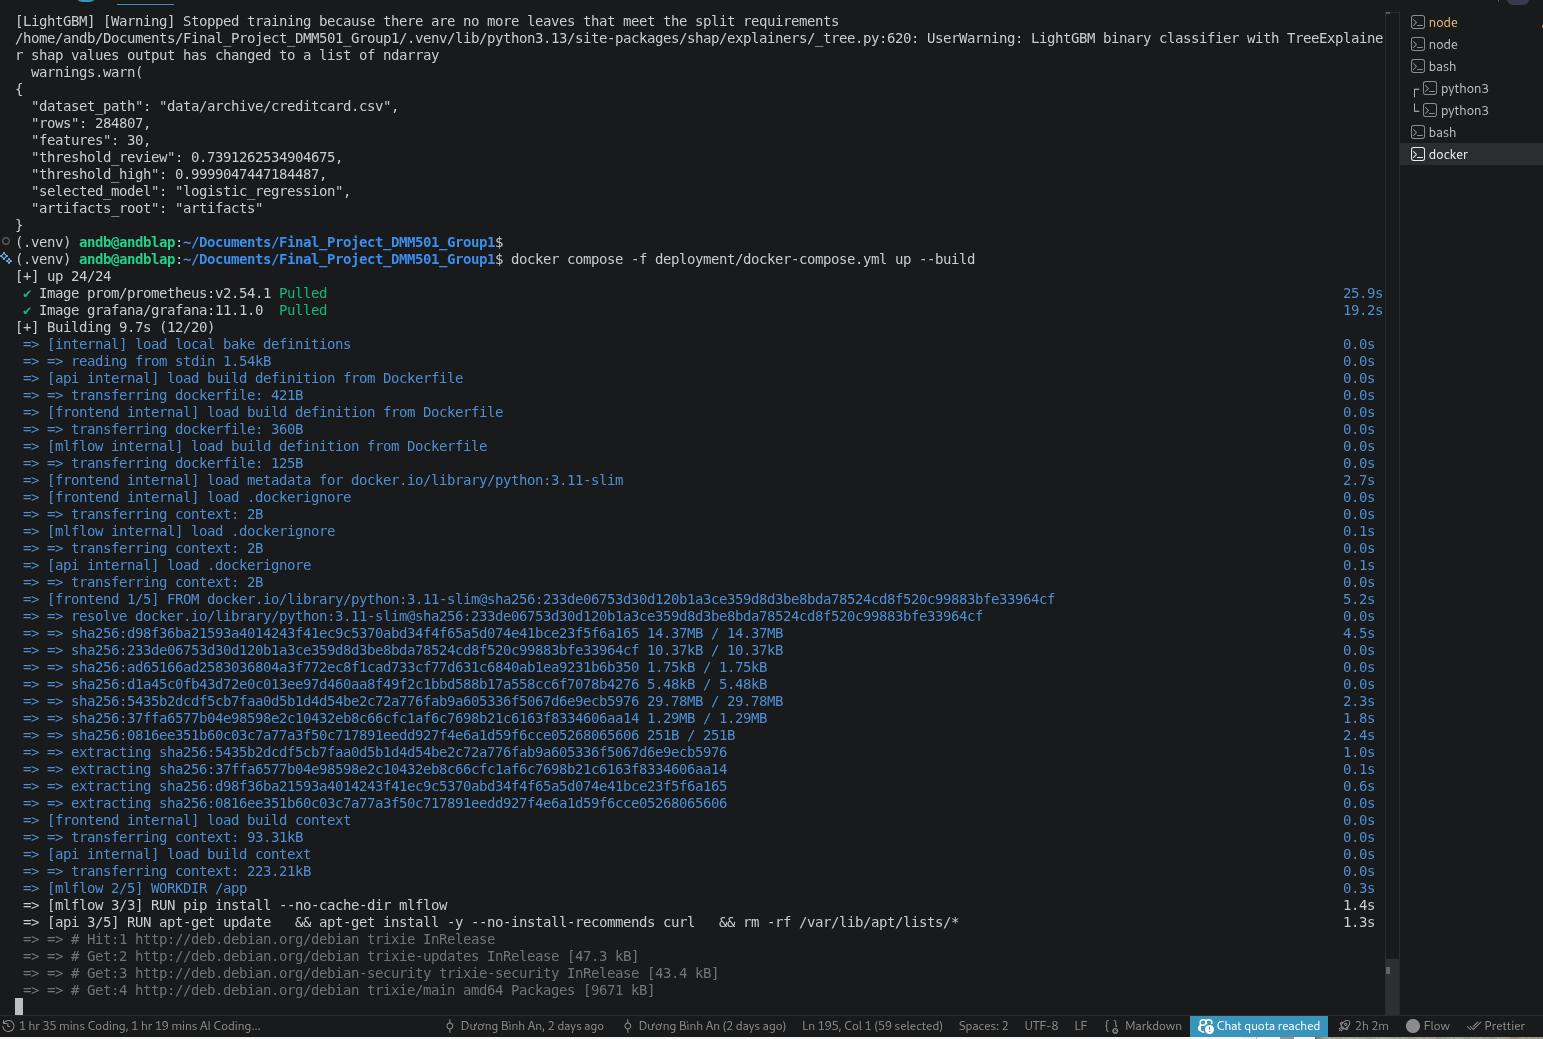
\includegraphics[width=0.92\linewidth]{../artifacts/deploys/docker-compose.png}
  \caption{Docker Compose stack evidence screenshot. Source: \code{artifacts/deploys/docker-compose.png}}
  \label{fig:docker_compose}
\end{figure}
\begin{figure}[H]
  \centering
  
\includegraphics[width=0.88\linewidth]{../artifacts/deploys/swagger-docs.png}
  \caption{Swagger UI screenshot for API endpoint verification. Source: \code{artifacts/deploys/swagger-docs.png}}
  \label{fig:swagger_docs}
\end{figure}

\subsection{Deployment contract (model + threshold)}
Compose sets \code{MODEL_PATH=/app/artifacts/models/final_model.joblib} and \code{FRAUD_THRESHOLD="0.99"}. The API loader reads \code{model_info.json} next to the model artifact to obtain \code{n_features}, feature names, dataset path, and selection timestamp.

\section{Testing \& CI/CD}
\subsection{Tests (evidence)}
\begin{itemize}
  \item Unit tests: \code{tests/unit/}
  \item Integration tests: \code{tests/integration/}
  \item Model/data tests: \code{tests/model/}, \code{tests/data/}
\end{itemize}
\textbf{Status:} \statusunverified{} execution in this report generation environment.

\subsection{GitHub Actions workflows (evidence)}
\begin{itemize}
  \item CI + coverage gate: \code{.github/workflows/ci.yml} (requires coverage \(\ge 80\%\))
  \item Docker build + compose config validation: \code{.github/workflows/docker.yml}
\end{itemize}

\section{Responsible AI}
Responsible AI documentation is provided in \code{RESPONSIBLE_AI.md}, including:
\begin{itemize}
  \item fairness limitations (no protected attributes in dataset)
  \item explainability via SHAP (LightGBM artifacts)
  \item privacy stance (avoid logging raw features; prefer aggregated metrics)
  \item ethical risks (false positives/false negatives) and mitigation strategies
\end{itemize}

\section{Limitations}
\subsection{Verified vs unverified in this report}
\begin{itemize}
  \item \statusverified{}: dataset presence; benchmark artifacts; figures; deploy metadata; frontend code; monitoring/deployment configuration files.
  \item \statusunverified{}: live API responses; running Compose stack; Grafana screenshots; executing tests and CI runs.
\end{itemize}

\subsection{Multiple artifact sets (do not conflate)}
This repository contains two artifact tracks:
\begin{itemize}
  \item Kaggle benchmark track under \code{artifacts/models/} with 30 features (used for deployment contract and dashboard).
  \item Synthetic training track under \code{artifacts/model.joblib}, \code{artifacts/model_info.json}, \code{artifacts/metrics_report.json} with 20 features (\code{data_source: synthetic:make_classification}).
\end{itemize}
This report's end-to-end demo contract uses the Kaggle benchmark track (30 features).

\section{Conclusion}
\subsection{End-to-end completeness (implementation)}
At demo scope, the repository implements: real dataset, reproducible benchmark pipeline producing artifacts, deployable model + threshold policy, serving API with metrics, frontend dashboard calling the real API, and monitoring/deployment configuration.

\subsection{Demo readiness (next evidence to capture)}
For submission-quality proof, capture:
\begin{itemize}
  \item real \code{/health}, \code{/predict}, \code{/metrics} outputs (JSON/text) while API is running
  \item frontend screenshot while stream is running (alerts + feed + chart)
  \item Grafana dashboard screenshot while streaming (optional, via Compose)
\end{itemize}

\section*{Appendix: System components status table}
\addcontentsline{toc}{section}{Appendix: System components status table}

\begin{longtable}{p{0.18\textwidth} p{0.37\textwidth} p{0.16\textwidth} p{0.24\textwidth}}
\toprule
\textbf{Component} & \textbf{Evidence} & \textbf{Status} & \textbf{How to verify} \\
\midrule
\endhead

Dataset & \code{data/archive/creditcard.csv}, \code{artifacts/reports/dataset_schema.json} & \statusverified{} & N/A \\
ML pipeline outputs & \code{src/pipelines/run_model_workflow.py}, \code{artifacts/reports/*}, \code{artifacts/figures/*} & \statusverified{} & Re-run workflow \\
Deployable model & \code{artifacts/models/final_model.joblib}, \code{artifacts/models/model_info.json} & \statusverified{} & Load via joblib (after deps) \\
API runtime & \code{src/api/main.py} + \code{tests/integration/*} & \statusunverified{} & Start Uvicorn + curl \\
Frontend runtime & \code{frontend/*}, screenshot \code{frontend_dashboard.png} & \statusunverified{} & Serve \code{frontend/} \\
Monitoring runtime & \code{deployment/prometheus/*}, \code{deployment/grafana/*} & \statusunverified{} & Run Compose \\
CI runs & \code{.github/workflows/*} & \statusunverified{} & Check GitHub Actions \\
\bottomrule
\end{longtable}

\end{document}
